\documentclass[10pt,letterpaper]{article}

\usepackage{cogsci}
\usepackage{pslatex}
\usepackage[natbibapa]{apacite}
\usepackage{auto-pst-pdf}
\usepackage{com.braju.graphicalmodels} \usepackage{com.braju.pstricks}
\catcode`\@=11%


\usepackage{enumitem}
\usepackage[tight,FIGBOTCAP]{subfigure}
\usepackage{graphicx}
%\usepackage{caption}
%\usepackage{subcaption}
\usepackage{sidecap}
\usepackage{amsmath}
\usepackage{pbox}

\setlength\intextsep{5pt}
\setlength{\belowcaptionskip}{-8pt}

\title{Modeling idiosyncratic preferences: How generative knowledge and expression frequency jointly determine language structure}
 
\author{{\large \bf Emily Morgan (eimorgan@ucsd.edu)} \\
  \AND {\large \bf Roger Levy (rlevy@ucsd.edu)} \\
  Department of Linguistics, UC San Diego, 9500 Gilman Drive,
  La Jolla, CA 92093-0108 USA}


\begin{document}

\maketitle


\begin{abstract}
Most models of choice in language focus on broadly applicable generative knowledge, treating item-specific variation as noise. Focusing on word order preferences in \emph{binomial expressions} (e.g. \emph{bread and butter}), we find meaning in the item-specific variation: more frequent expressions have more polarized (i.e. frozen) preferences. Of many models considered, only one that takes expression frequency into account can predict the language-wide distribution of preference strengths seen in corpus data. Our results support a gradient trade-off in language processing between generative knowledge and item-specific knowledge as a function of frequency.

\textbf{Keywords:} 
Bayesian modeling; binomial expression; frequency; word order
\end{abstract}

\section{Introduction}
A pervasive question in language processing research is how we reconcile generative knowledge with idiosyncratic properties of specific lexical items. In many cases, the generative knowledge is the primary object of study, while item-specific idiosyncrasies are treated as noise. For instance, in modeling the dative alternation, \citet{Bresnan:2007td} take care to demonstrate that effects of animacy, givenness, etc. on structure choice hold even after accounting for biases of individual verbs. But the verb biases themselves are not subject to any serious investigation. Here we present evidence that patterns within the item-specific variation are meaningful, and that by modeling this variation, we not only obtain better models of the phenomenon of interest, we also learn more about language structure and its cognitive representation.

%A central question in the theory of language processing is how generative linguistic knowledge interacts with formulaic language. A trade-off between these knowledge sources can be found at multiple levels of linguistic processing, including in morphology (i.e. whether morphologically complex forms are always decomposed or whether they are stored holistically) and in sentence processing (i.e. likewise whether multi-word expressions are processing combinatorially or holistically). This question has typically been asked from the perspective of an individual's lexical knowledge and synchronic language processing. For example, \citet{Morgan:uMm0l0Ja} have demonstrated a trade-off between reliance upon generative constraints and reliance upon stored chunks for multi-word expressions dependent upon expression frequency.
%
%Another take on this question comes from a evolutionary or language-structure perspective: what we know about how stored forms enter into and evolve within the language can also constrain our theories of language learning and representation by elucidating what types or properties of stored forms must be learned, and under what conditions. Specifically, we will argue that a rational, gradient trade-off between compositional knowledge and stored formulaic language is necessary to explain facts about language structure.

Specifically, we will develop a model of word order preferences for \emph{binomial expressions} of the form \emph{X and Y} (i.e. \emph{bread and butter} preferred over \emph{butter and bread}). Binomial ordering preferences are in part determined by generative knowledge of violable constraints which reference the semantic, phonological, and lexical properties of the constituent words \citep[e.g. short-before-long;][]{Cooper:1975uz,McDonald:1993wq}, but speakers also have idiosyncratic preferences for known expressions \citep{SiyanovaChanturia:2011ep,Morgan:uMm0l0Ja}. Binomial expressions are a useful test case for modeling idiosyncracies because their frequencies can be robustly estimated from the Google Books n-grams corpus \citep{Lin:2012te}. Here we will demonstrate that explicitly modeling these expressions' idiosyncrasies both produces a better predictive model for novel expressions and also constrains our theory of these expressions' cognitive representations.

Specifically, we identify two reasons why such a model is advantageous:
\subsection{1. Models identify both rules and exceptions.}
One intrinsic reason that modeling idiosyncrasies is advantageous is because identifying exceptions can help identify rules. In a traditional linguistic setting (e.g. identifying rules for past tense formation), we rely upon intuition to determine what is the grammatical rule and which verbs should be treated as exceptions. In the case of binomial expressions, we likewise expect there to be exceptions to the rules, particularly for frequent expressions. For example, there is in general a strong constraint to put men before women; however, \emph{ladies and gentlemen} is preferred over the reverse due to its conventionalized formal use. But compared with past tense formation, the rules that determine binomial ordering are far more complex and gradient, such that using traditional linguistic analysis to determine the full set of rules is not viable. In this case, we require our model not only to identify what the rules are but simultaneously to determine which expressions must be treated as exceptions. Having such a model is useful for empirical cognitive science, e.g. for disentangling the effects of people's generative knowledge from effects of their item-specific linguistic experience on language processing \citep{Morgan:uMm0l0Ja}.

\subsection{2. Models relate cognitive representations to language-wide structure.}
As a further benefit, models can help us understand how structural properties of the language relate to people's cognitive linguistic representations. In particular, let us look at the distribution of preferences for binomial expressions taken from a subset of the Google Books corpus (described later in Creating the Corpus.) Each binomial can be assigned a preference strength corresponding to how frequently it appears in alphabetical order, from 0 (always in non-alphabetical order) to 0.5 (perfectly balanced) to 1 (always alphabetical). Binomials which always or nearly always appear in one order are said to be \emph{frozen}. The distribution of preference strengths is shown in Figure \ref{fig:corpus-hist}. Preferences have a multimodal distribution with modes at the extremes as well as around 0.5. This distribution poses a challenge to standard models of binomial preferences. As we will show later, standard models predict only a single mode around 0.5. In other words, the true distribution of binomial expressions includes more frozen binomials than standard models predict. As we develop a model that accounts for this multimodal distribution, we will see that this language-structural fact puts constraints on our theories of individuals' cognitive representations of binomial expressions.

In the remainder of this paper, we first describe how we developed a new corpus of binomial expressions. We then explore a variety of models with differing levels of ability to model item-specific idiosyncrasies. Finally, we return to the issue of how these models inform us about cognitive representations of language.

\begin{figure}[h]
\centering
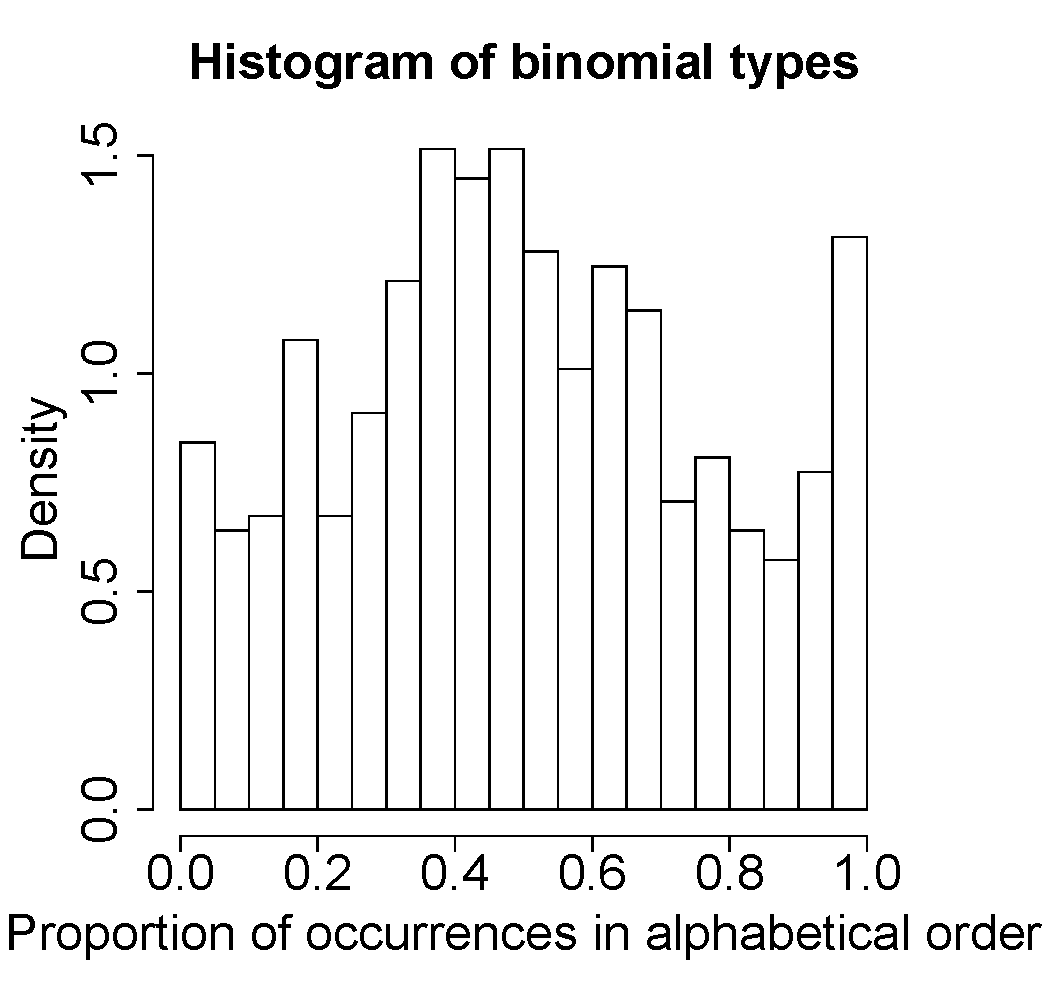
\includegraphics[scale=.3]{corpus-hist.pdf}
\vspace{-10pt}
\caption{Binomial preferences are multimodally distributed in corpus data}
\label{fig:corpus-hist}
\end{figure}


\section{Creating the Corpus} \label{corpus}
We extracted all \emph{Noun-and-Noun} binomials from the parsed section of the Brown corpus \citep{Treebank:tt} using the following Tregex \citep{Levy:2006us} search pattern:
\begin{verbatim}/^N/=top < (/^NN/ !$, (/,/ > =top) .
((CC <: and > =top) . (/^NN/ > =top)))\end{verbatim}
This pattern finds all Noun-\emph{and}-Noun sequences dominated by a Noun Phrase which are not preceded by a comma (to exclude the final pair in lists of more than two elements), a total of 1280 tokens.

Binomials were coded for a variety of constraints, originally described by \citet{Benor:2006gv} but restricted to the subset determined to be most relevant for predicting ordering preferences by \citet{Morgan:uMm0l0Ja}:
\begin{description}[noitemsep,style=unboxed,leftmargin=0cm]
  \item[Length] The shorter word (in syllables) comes first, e.g. \emph{abused and neglected}.
  \item[No final stress] The final syllable of the second word should not be stressed, e.g. \emph{abused and neglected}.
  \item[Lapse] Avoid unstressed syllables in a row, e.g. \emph{FARMS and HAY-fields vs HAY-fields and FARMS}
  \item[Frequency] The more frequent word comes first, e.g. \emph{bride and groom}.
  \item[Formal markedness] The word with more general meaning or broader distribution comes first, e.g. \emph{boards and two-by-fours}.
  \item[Perceptual markedness] Elements that are more closely connected to the speaker come first. This constraint encompasses \citeauthor{Cooper:1975uz}'s \citeyearpar{Cooper:1975uz} `Me First' constraint and includes numerous subconstraints, e.g.: animates precede inanimates; concrete words precede abstract words; e.g. \emph{deer and trees}.
  \item[Power] The more powerful or culturally prioritized word comes first, e.g. \emph{clergymen and parishioners}.
  \item[Iconic/scalar sequencing] Elements that exist in sequence should be ordered in sequence, e.g. \emph{achieved and maintained}.
  \item[Cultural Centrality] The more culturally central or common element should come first, e.g. \emph{oranges and grapefruits}.
  \item[Intensity] The element with more intensity appears first, e.g. \emph{war and peace}.
%  \item[Pragmatic] Catch-all constraint for influences of the local context, which---unlike other constraints---would not generally hold constant across occurrences of this word pair. In particular, an element that has been previously mentioned should come first. (Active for 51 tokens.)
\end{description}
The metrical constraints, Length and No final stress, were automatically extracted from the CMU Pronouncing Dictionary \citeyearpar{TheCMUPronouncing:ZV2ODMTE}, augmented by manual annotations when necessary. Word frequency was taken from the Google Books corpus, counting occurrences from 1900 or later. Semantic constraints were hand coded by two independent coders (drawing from the first author and two trained research assistants). Discrepancies were resolved through discussion.
%All except Cultural Centrality and Intensity have been described and used previously. These two constraints were introduced on the basis of the coders' early experience to resolve conflicts in the original constraint definitions used by \citet{Benor:2006gv}, specifically for cases where the same type of semantic relationship could be classified under multiple constraint definitions. For the sake of this type of corpus analysis, it is better to have a proliferation of constraints than too few constraints. In our analysis, it will always be possible for two constraints to be weighted equally (e.g. if it turns out that we have unnecessarily separated out what is underlyingly one constraint into two constraints), but to unfoundedly collapse two constraints would prevent us from ever distinguishing between them in our analyses. Thus we err on the side of having more constraints rather than fewer.

%Cultural Centrality was formerly coded under either Perceptual Markedness or Power. Itensity was formerly coded under Power (predicting more intense first), Formal Markedness (in cases where one item is a more intense subset of the other, thus predicting more intense second, e.g. ``apprehension and fear''), or Iconic Sequencing (in cases where the elements exist on a scale of intensity, also predicting more intense second, e.g. ``sparks and flames'').

For each binomial, we obtained the number of occurrences in both possible orders in the Google Books corpus from 1900 or later. Items containing proper names, those with errors in the given parses, those whose order was directly affected by the local context (e.g. one element had been mentioned previously), and those with less than 1000 total occurrences across both orders were excluded from analysis, leaving 594 binomial expression types.
% those for which the Pragmatic constraint applied

\section{Models}
We will develop four models of binomial ordering preferences: a standard logistic regression, a mixed-effects logistic regression, and two hierarchical Bayesian beta-binomial models. All are based on the idea of using logistic regression to combine the constraints described above in a weighted fashion to produce an initial preference estimate for each binomial. The models differ in whether and how they explicitly model the fact that true preferences will be distributed idiosyncratically around these estimates. The standard logistic regression includes no explicit representation of item-specific idiosyncrasies. The mixed-effect logistic regression includes random intercepts which account for item-specific idiosyncrasies, but which are constrained to be distributed normally around the initial prediction. The two Bayesian models assume that item-specific preferences are drawn from a beta distribution whose mean is determined by the initial prediction. In the first of these models, the concentration of the beta distribution is fixed, while in the second, it varies with the frequency of the binomial in question. 

\subsection{Evaluation}
One obvious criterion for evaluating a model is how well it predicts known binomial preferences (i.e. the corpus data). For this, we report $R^{2}(X,\hat{X})$ as well as mean L1 error, $\frac{1}{N}\Sigma_{i=1}^{N} \left| \hat{x_i} - x_i\right|$, where $\hat{x_i}$ is the model prediction for how often binomial $i$ occurs in a given order, and $x_i$ is the true corpus proportion.

In addition to considering model predictions for each individual item, we want to consider the overall distribution of preferences within the language. As we will see, a model can provide good predictions for individual items without correctly capturing the language-wide multimodal distribution of these expressions' preference strengths. Thus our second desideratum will be the shape of the histogram of expression preferences.

%\subsection{By tokens} %don't include this in the cogsci paper
%Following \citet{Benor:2006gv} and \citet{Morgan:uMm0l0Ja}, we start by developing a logistic regression model that predicts preferences from abstract constraints. For a given word pair \emph{(A,B)}, a logistic regression model can predict the probability that a binomial expression will be realized as \emph{A and B}. The easiest way to train this model is by tokens, e.g. for every binomial in our corpus, for every instance of it in the google books corpus, we count this as a separate data point.
%
%For this an all future models, outcomes are coded as 1 for alphabetical order and 0 for non-alphabetical. Constraints are positive if they favor alphabetical and negative if they favor the reverse.
%
%% Build some big omnibus table with constraint weights and correlations of outcomes with corpus data (and maybe other error measures?) for all the models.
%
%Results can be seen in Table \ref{t:omni}. Correlation of outcomes with corpus data is ? and other error measures are ?. Results are visualized in Figures \ref{f:types-scatter} and \ref{f:types-hist}. Although this model has a reasonable correlation and error statistics, we can do better (as we will see) and it fails to capture the correct histogram shape.
%
%One problem with a by tokens model, noted by \citet{Benor:2006gv}, is that there are a small number of items that occur very frequently that may be skewing the statistics. To avoid this, we develop a by types model.

\subsection{Logistic regression}\label{logistic}
Logistic regression is the standard for modeling syntactic alternations, both for binomial expressions specifically \citep[e.g.][]{Benor:2006gv,Morgan:uMm0l0Ja} as well as other syntactic alternations \citep[e.g.][]{Bresnan:2007td,FlorianJaeger:2010hl}. Thus we begin by constructing a baseline logistic regression model. \citeauthor{Benor:2006gv} have argued that one should train such a model on binomial types rather than binomial tokens because otherwise a large number of tokens for a small number of overrepresented types can skew the results. While agreeing with this logic, we note that to train only a single instance of each type is to ignore a vast amount of data about the gradient nature of binomial preferences. As a compromise, we instead train a model on binomial tokens, using token counts from the Google Books corpus, with each token weighted in inverse proportion to how many tokens there are for that binomial type, i.e. a type with 1000 tokens will have each token weighted at 1/1000. In this way, we preserve the gradient information about ordering preferences (via the diversity of outcomes among tokens) while still weighting each type equally. The constraints described above are used as predictors. Outcomes are coded as whether or not the binomial token is in alphabetical order.

For this and all future models, predictions are generated for all training items using 20-fold cross validation. Results for all models can be seen in Figure \ref{fig:models}. While the logistic regression model does a reasonable job of predicting preferences for individual items, it does not capture the multimodal distribution of preference strengths seen in the corpus data. We proceed to consider models in which item-specific idiosyncrasies are modeled explicitly.


\begin{figure*}[htb]
  \begin{tabular}{p{0.75in}ccc}
  Logistic regression & \pbox[c]{\textwidth}{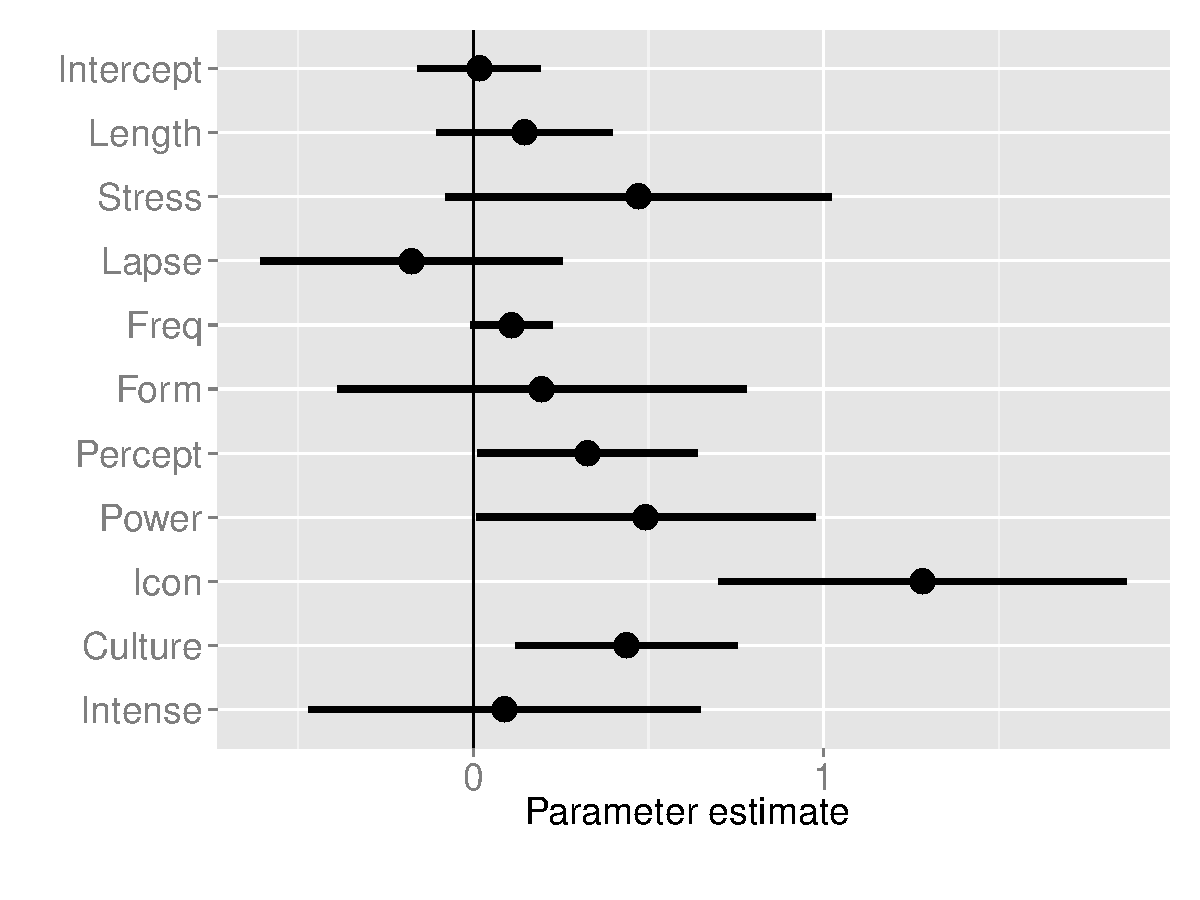
\includegraphics[scale=.35]{model-logistic.pdf}} & \pbox[c]{\textwidth}{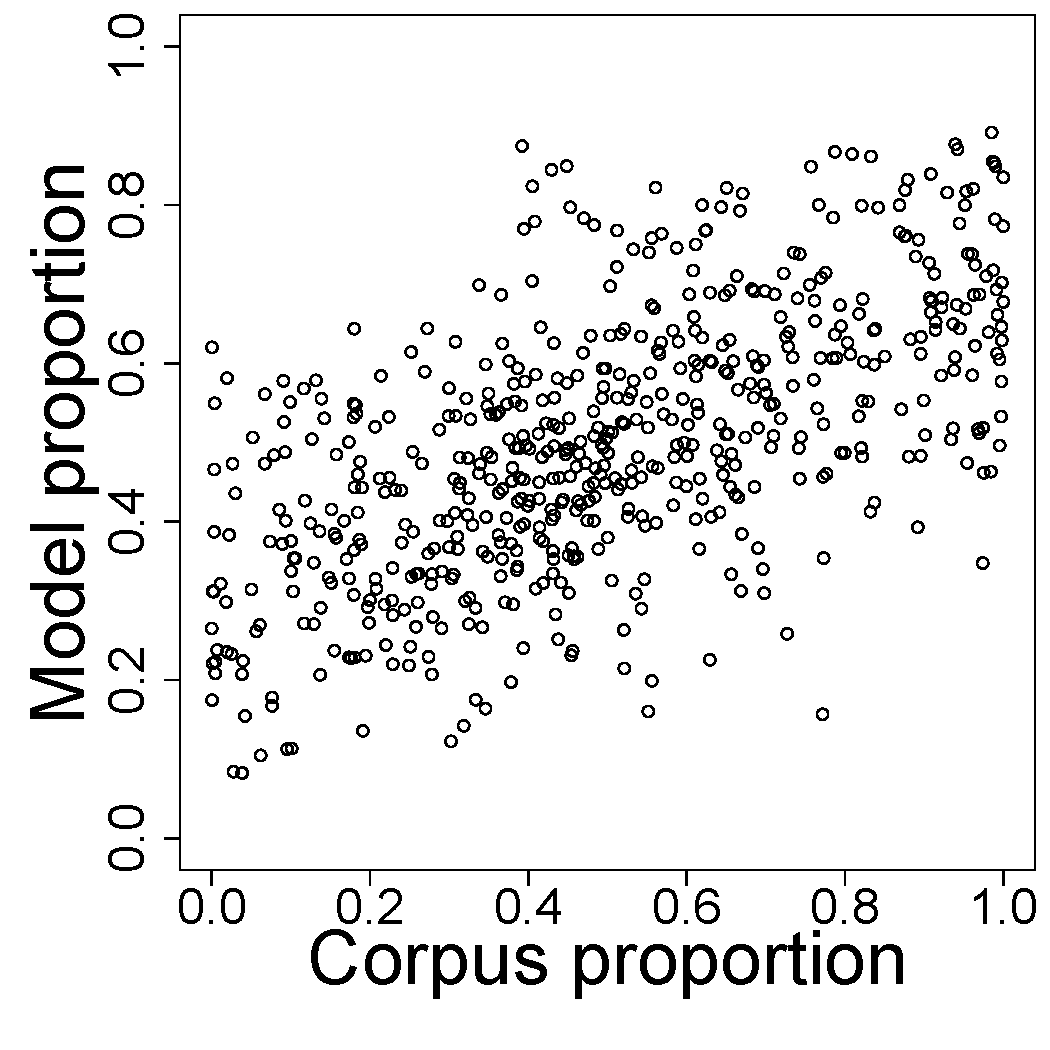
\includegraphics[scale=.2]{logistic-scatter.pdf}\\L1$ = 0.169$ (0.006)\\$R^{2}=0.368$ (0.021)} & \pbox[c]{\textwidth}{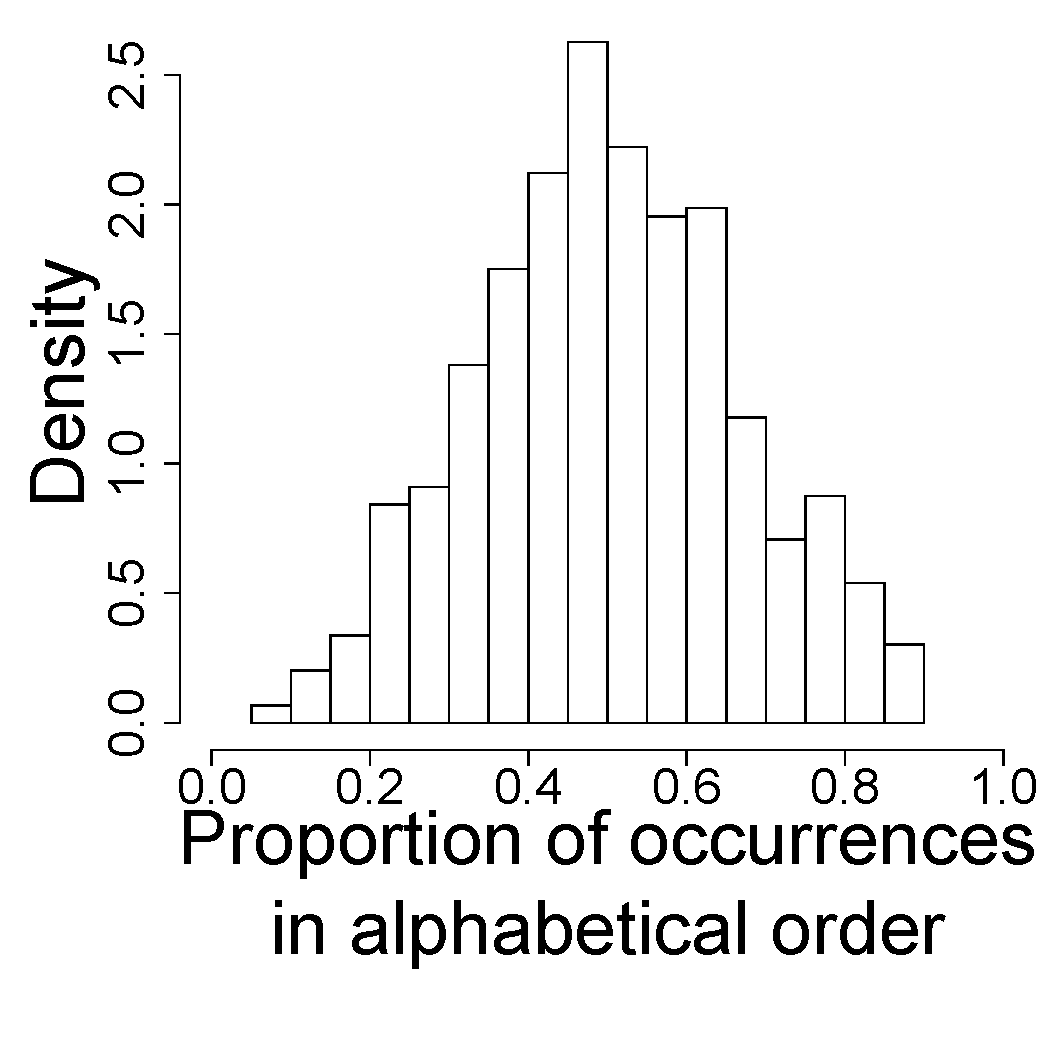
\includegraphics[scale=.2]{logistic-hist.pdf}} \\
  Mixed-effects regression with random intercept & \pbox[c]{\textwidth}{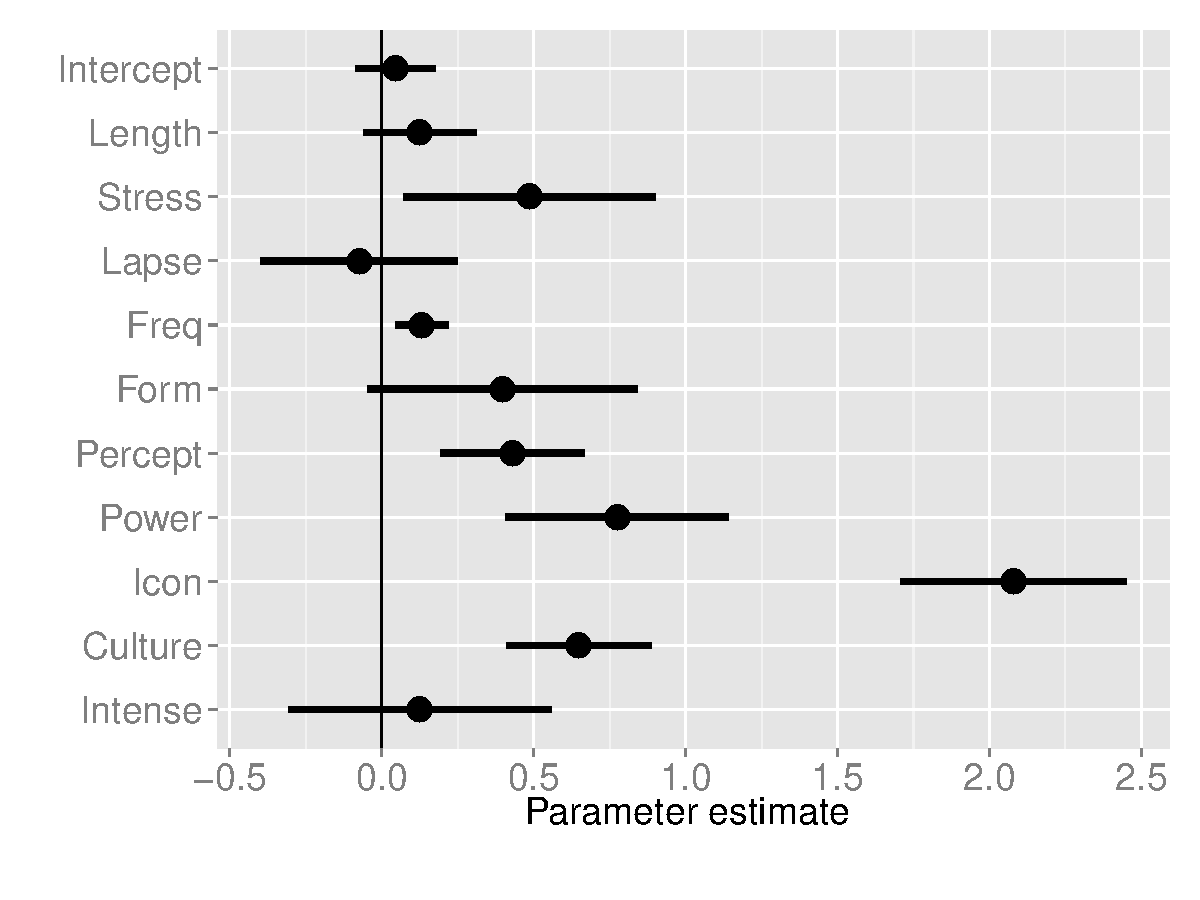
\includegraphics[scale=.35]{model-random.pdf}} & \pbox[c]{\textwidth}{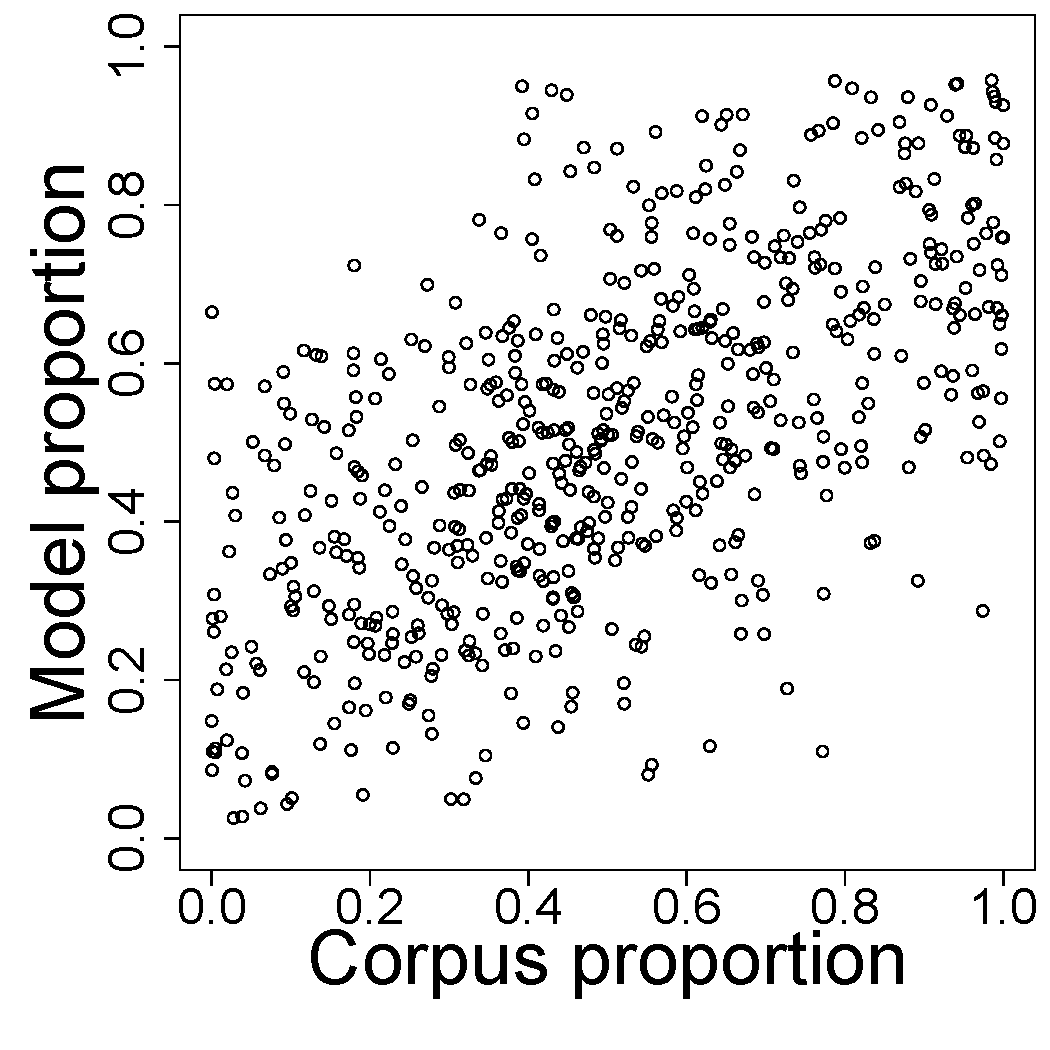
\includegraphics[scale=.2]{random-scatter.pdf}\\L1$ = 0.173$ (0.006)\\$R^{2}=0.355$ (0.022)} & \pbox[c]{\textwidth}{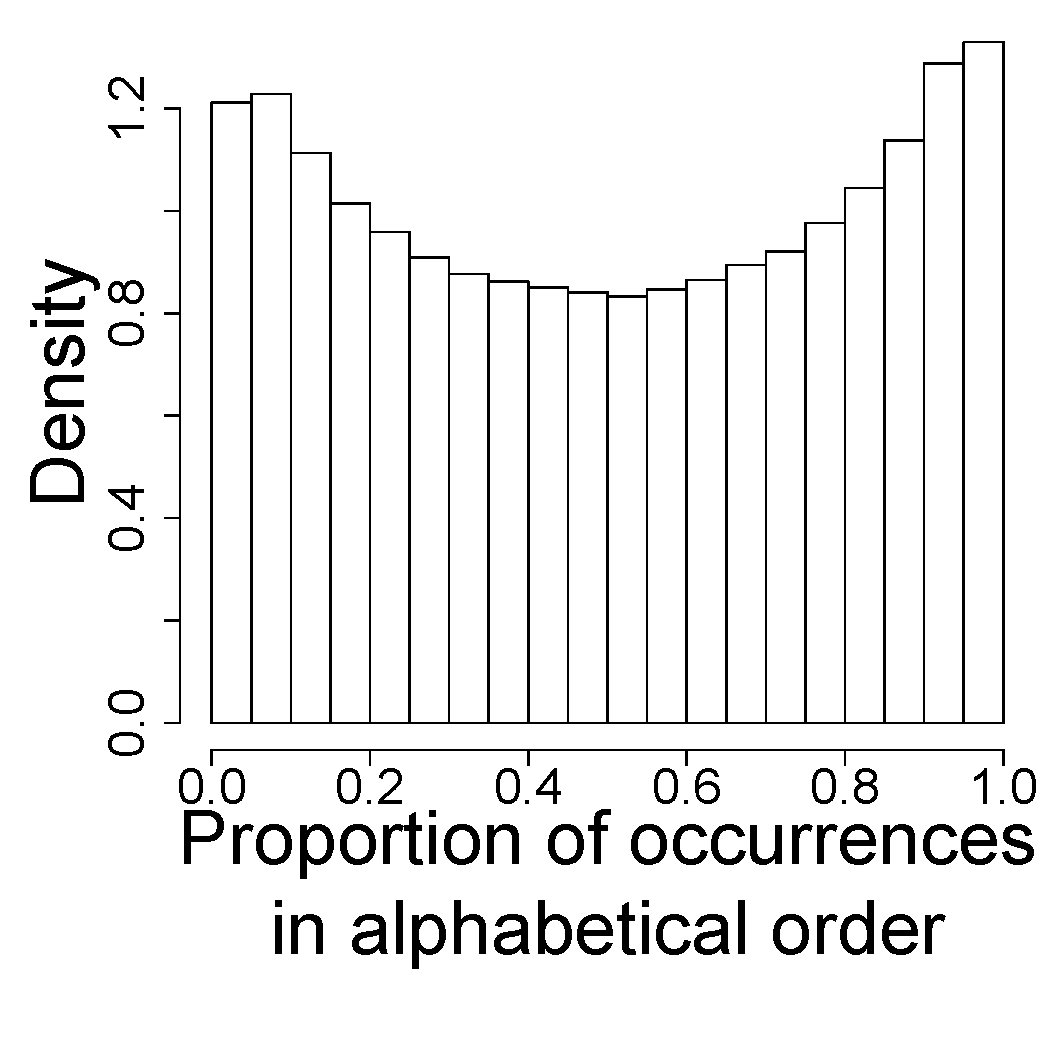
\includegraphics[scale=.2]{random-hist.pdf}} \\
  Beta-binomial model & \pbox[c]{\textwidth}{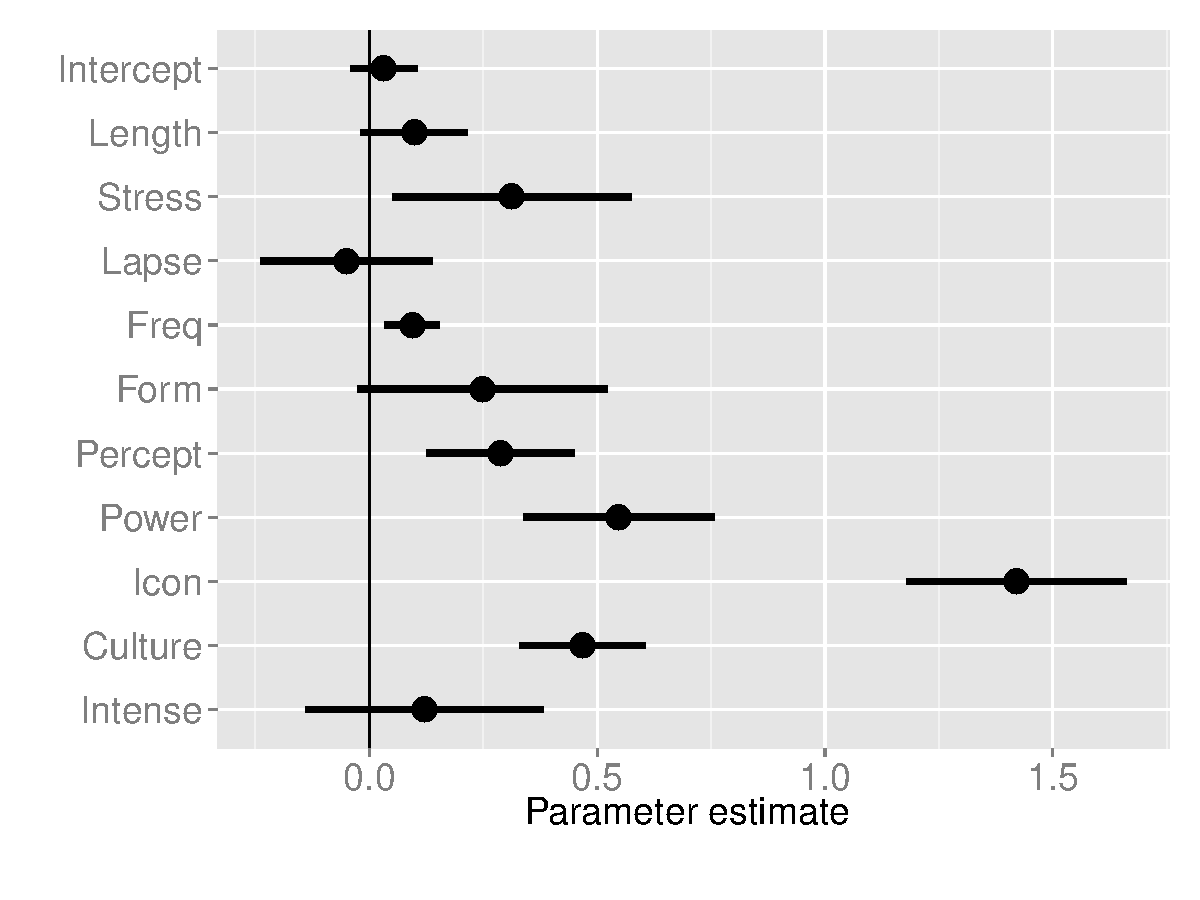
\includegraphics[scale=.35]{model-betabin.pdf}} & \pbox[c]{\textwidth}{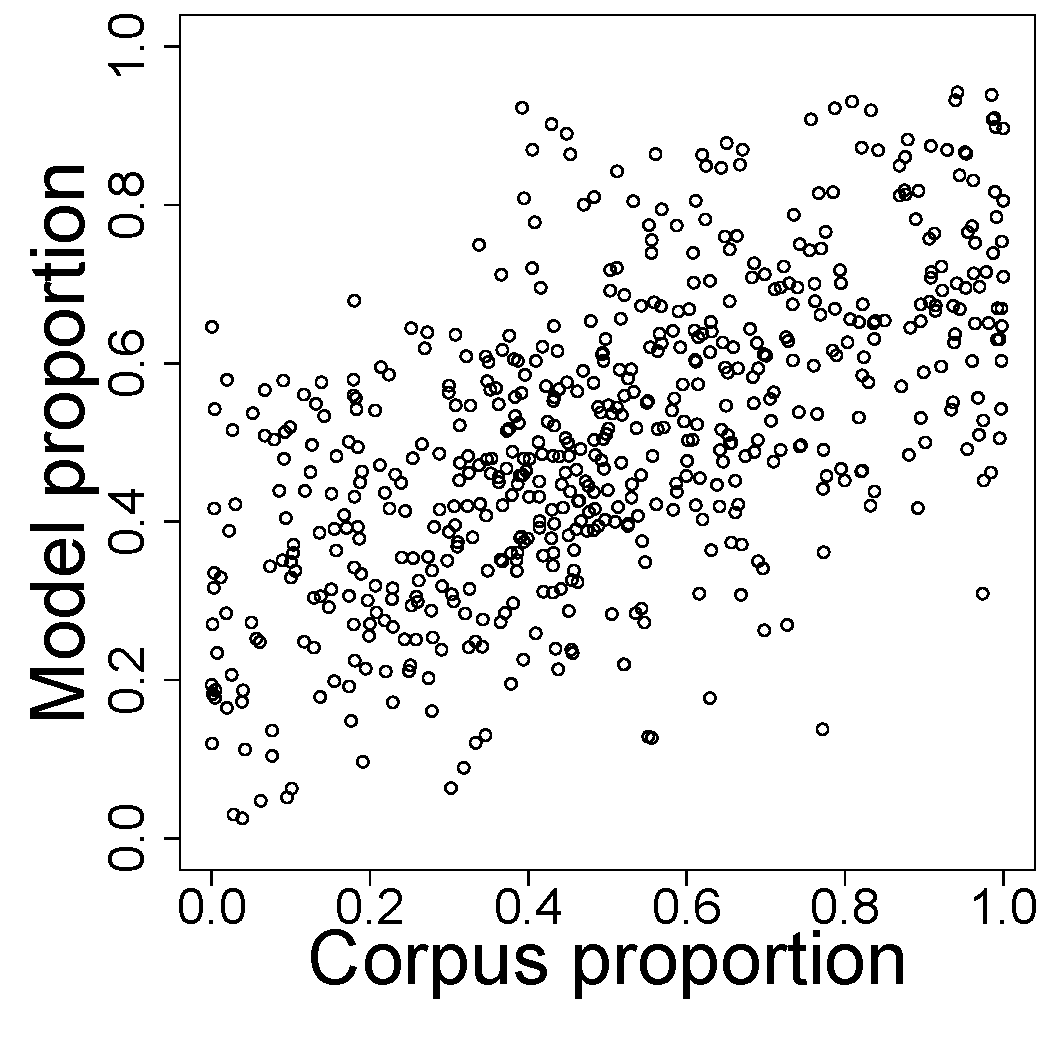
\includegraphics[scale=.2]{betabin-scatter.pdf}\\L1$ = 0.170$ (0.003)\\$R^{2}=0.367$ (0.020)} & \pbox[c]{\textwidth}{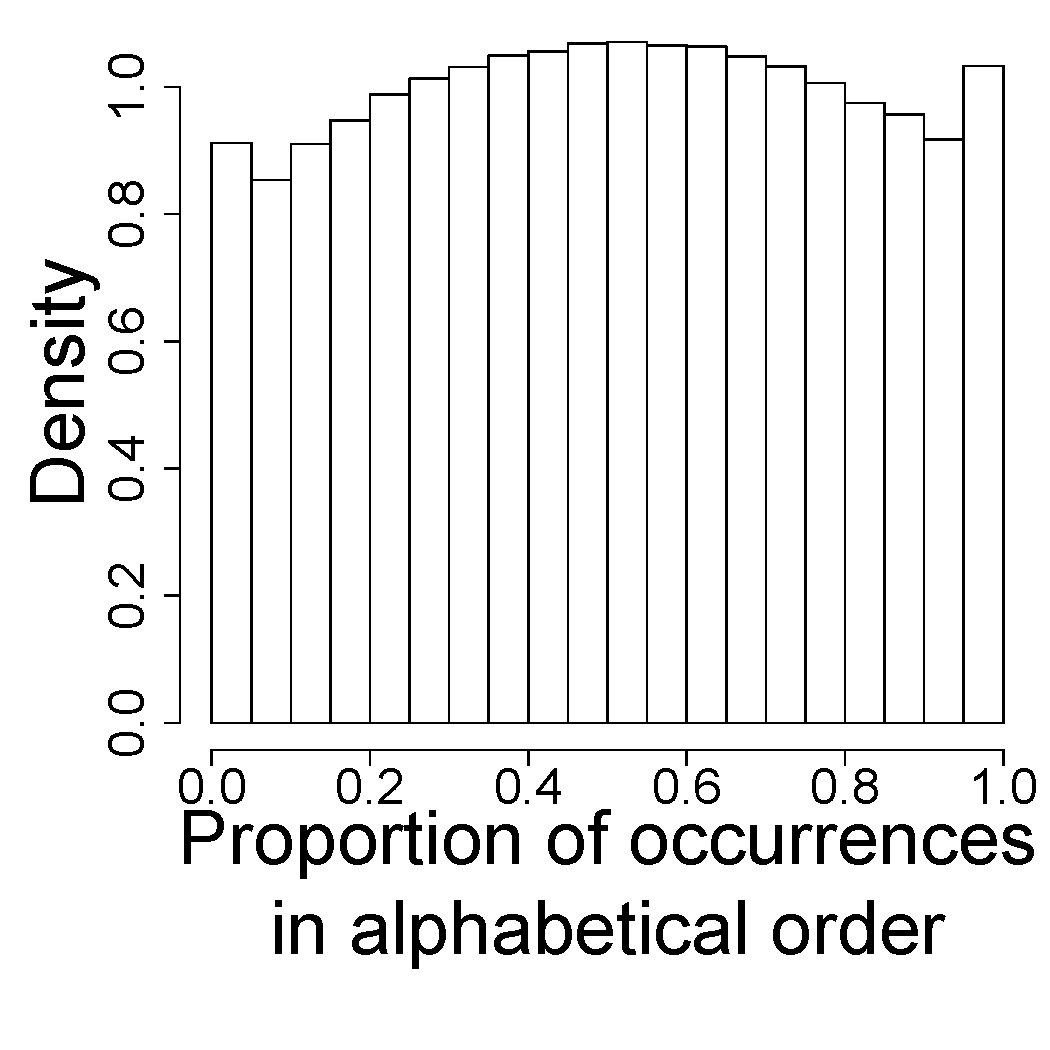
\includegraphics[scale=.2]{betabin-hist.pdf}} \\
  Beta-binomial model with variable concentration & \pbox[c]{\textwidth}{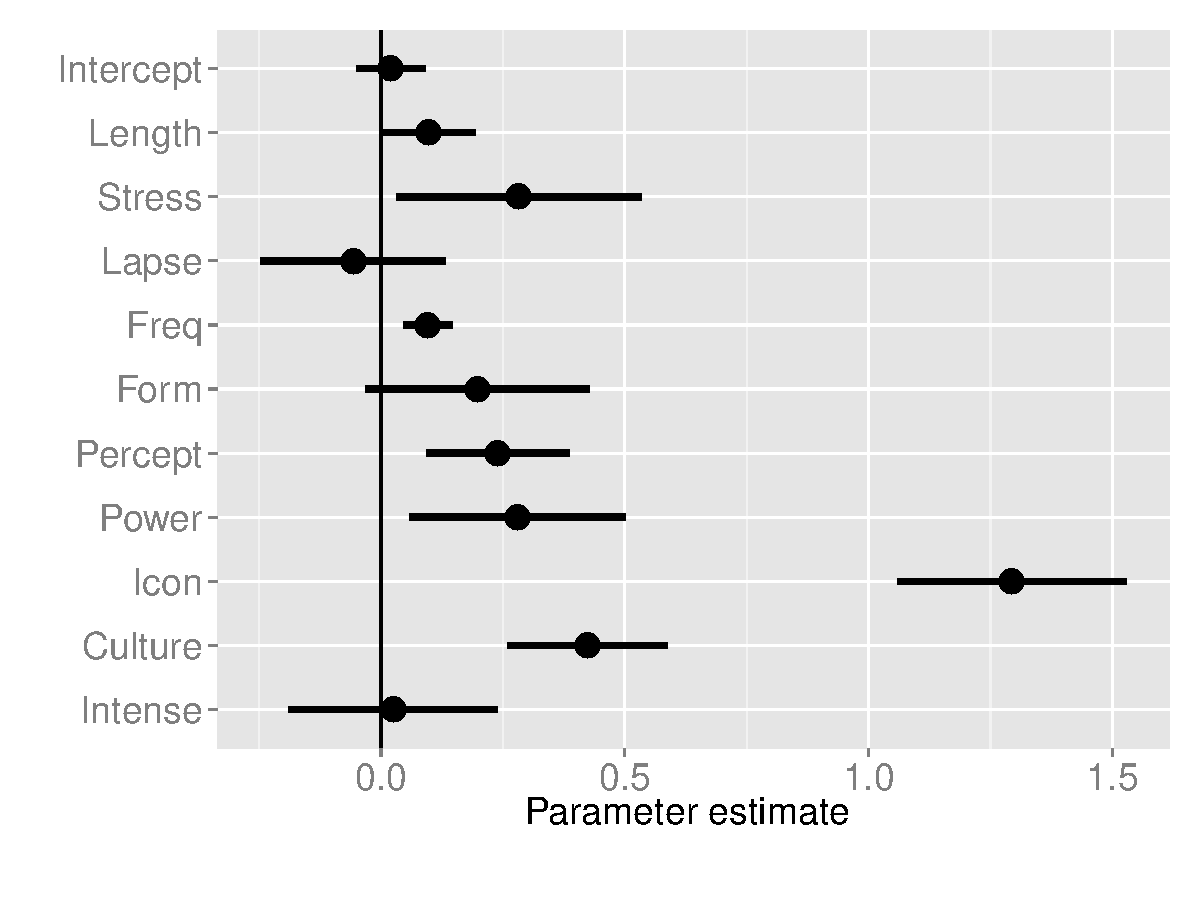
\includegraphics[scale=.35]{model-betabin-nu.pdf}} & \pbox[c]{\textwidth}{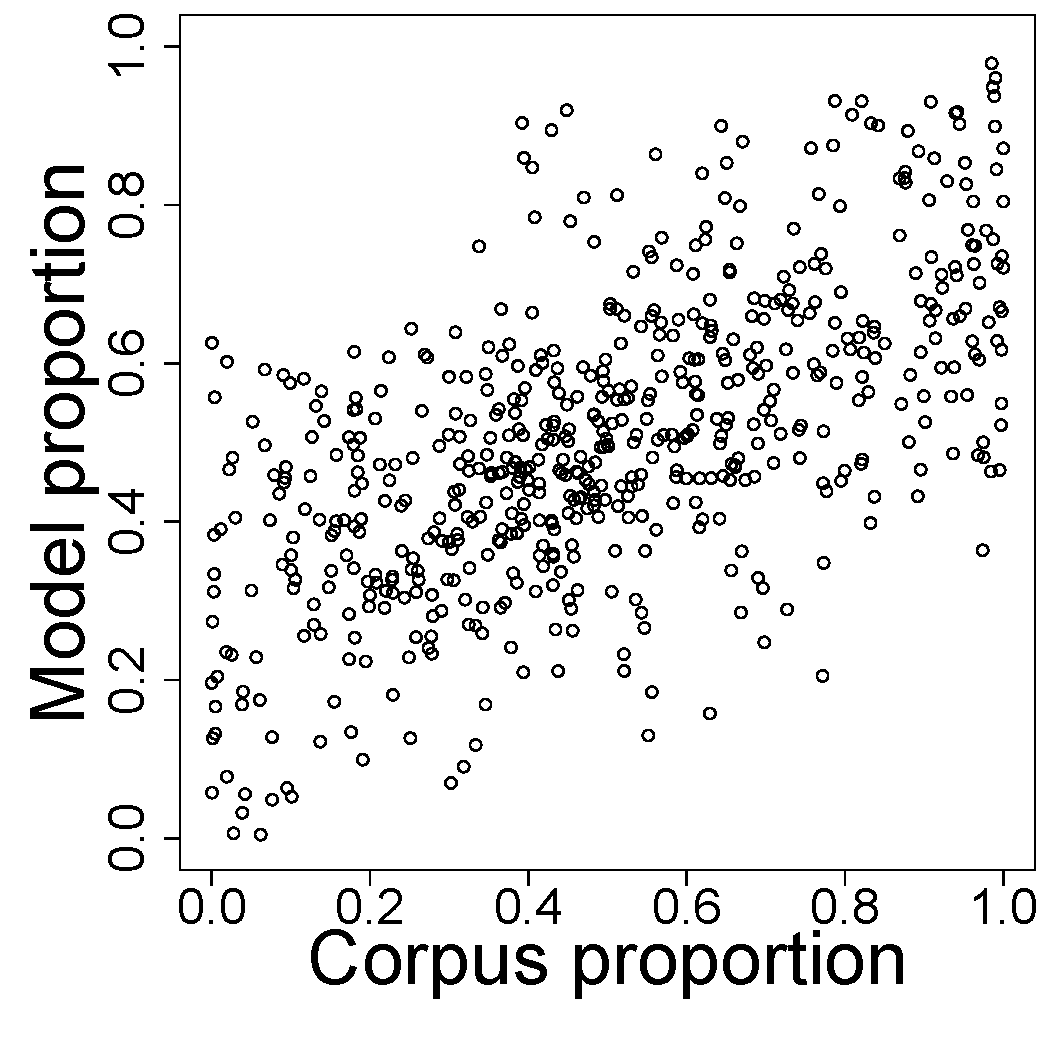
\includegraphics[scale=.2]{betabin-nu-scatter.pdf}\\L1$ = 0.166$ (0.003)\\$R^{2}=0.381$ (0.021)} & \pbox[c]{\textwidth}{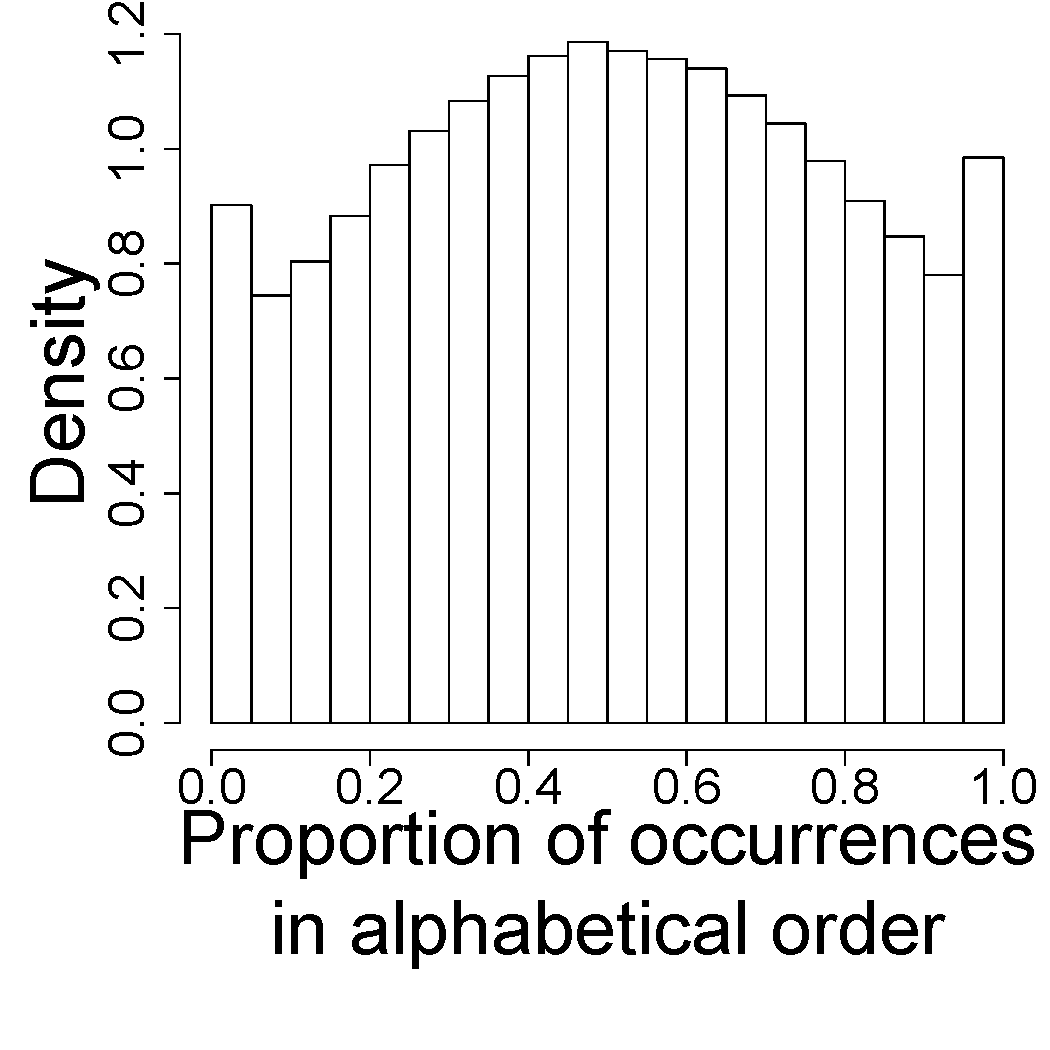
\includegraphics[scale=.2]{betabin-nu-hist.pdf}} \\
  & (a) & (b) & (c) \\
  \end{tabular}
  \caption{For each of our four models, we display: (a) Parameter estimates for the logistic regression component. Dots show point estimates with bars indicating standard errors. (b) Predictions for each item, as well as mean by-type L1 error and $R^{2}$ with by-fold standard errors. (c) Language-wide predicted distribution of preference strengths.}\label{fig:models}
\end{figure*}

%\begin{figure}[h]
%\centering
%\subfigure{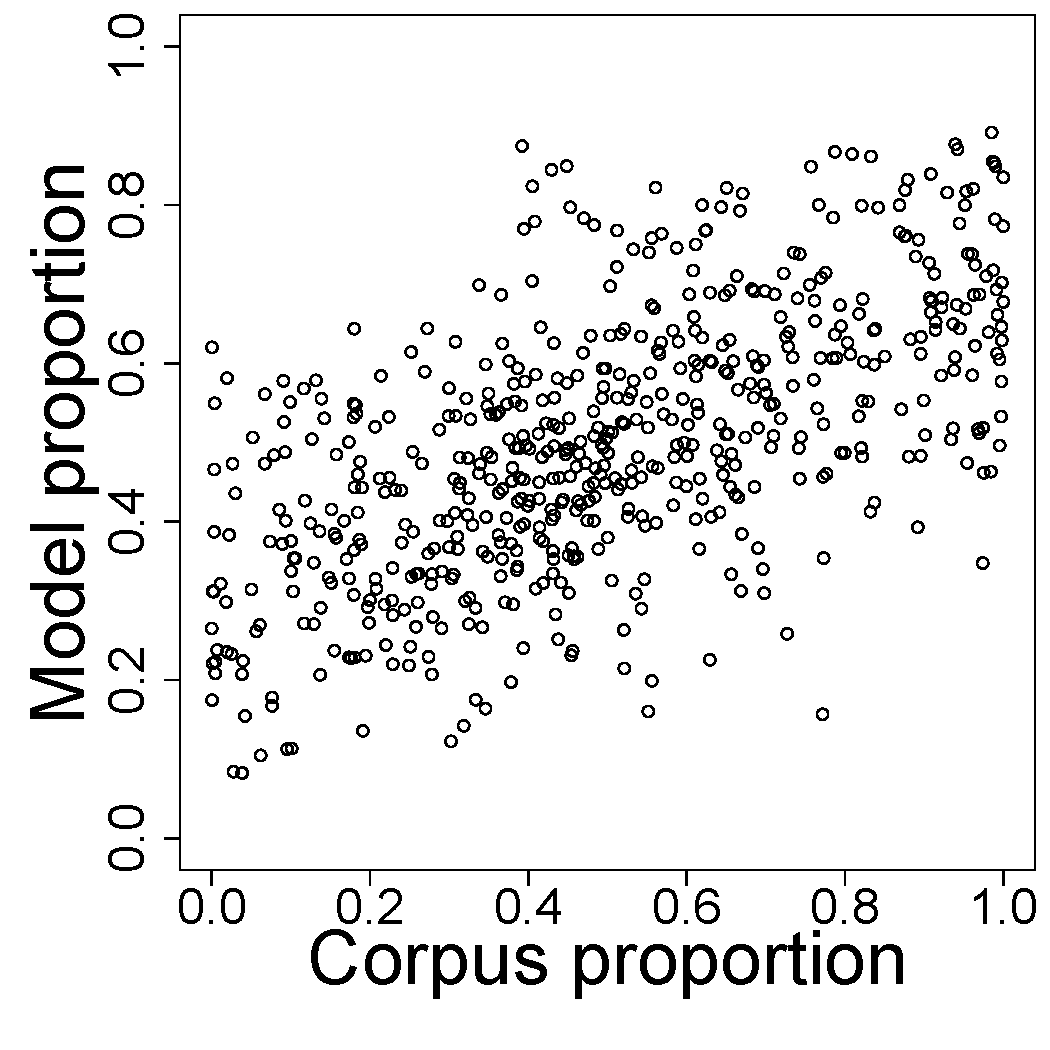
\includegraphics[scale=.25]{logistic-scatter.pdf}\label{fig:logistic-scatter}}
%\subfigure{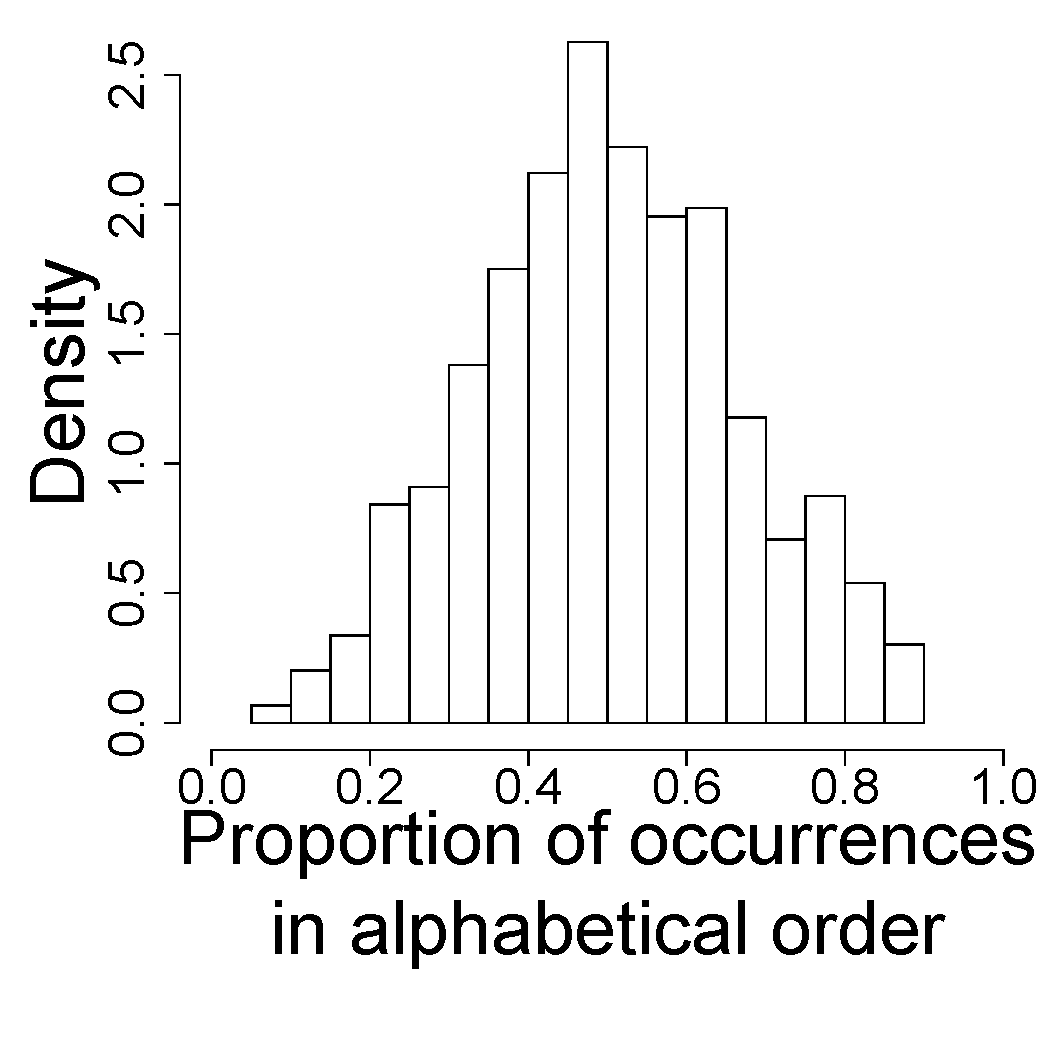
\includegraphics[scale=.2]{logistic-hist.pdf}\label{fig:logistic-hist}}
%\vspace{-10pt}
%\caption{Logistic regression results}
%\label{fig:logistic}
%\end{figure}
%
%\begin{figure*}[tb]
%\centering
%\subfigure[][Logistic regression]{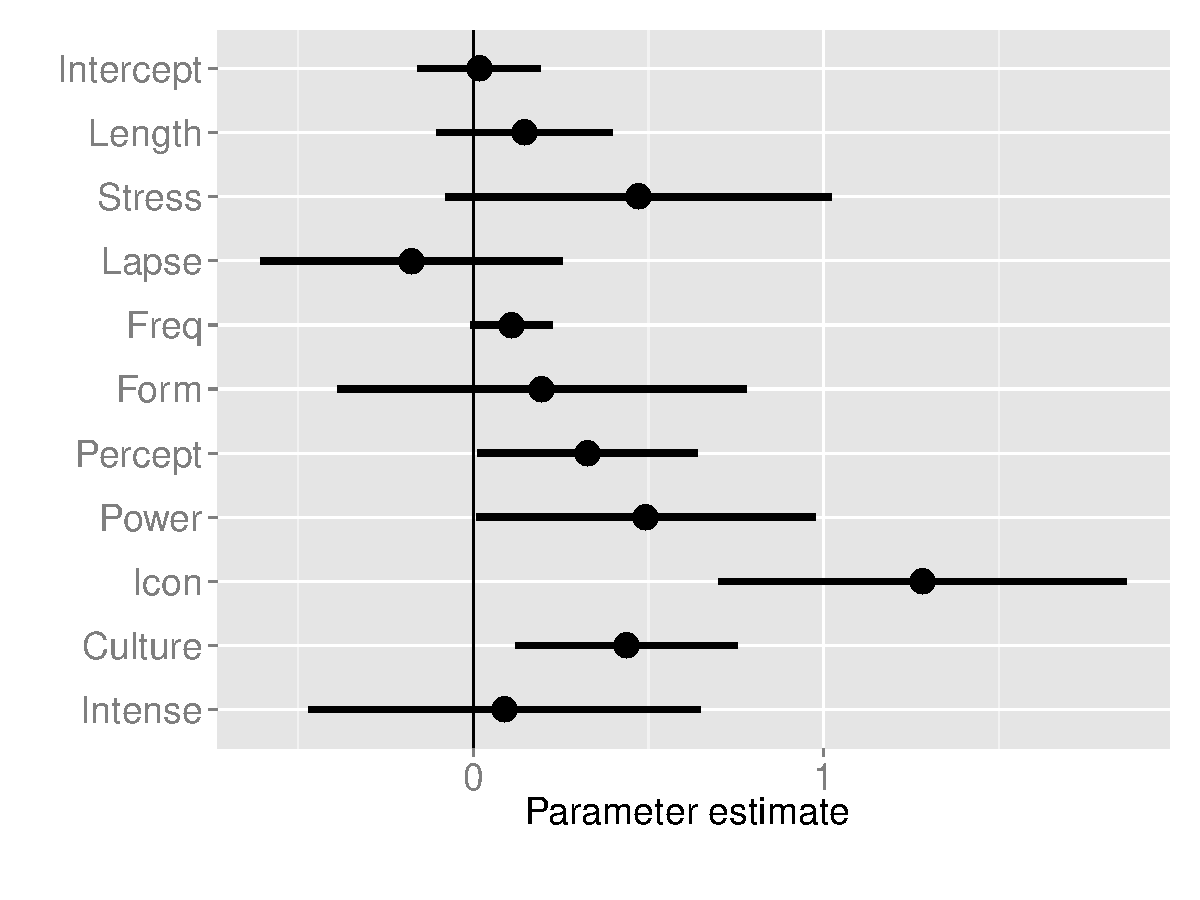
\includegraphics[scale=.35]{model-logistic.pdf}\vspace{-10pt}\label{fig:m-logistic}}
%\subfigure[][Logistic regression with random intercept]{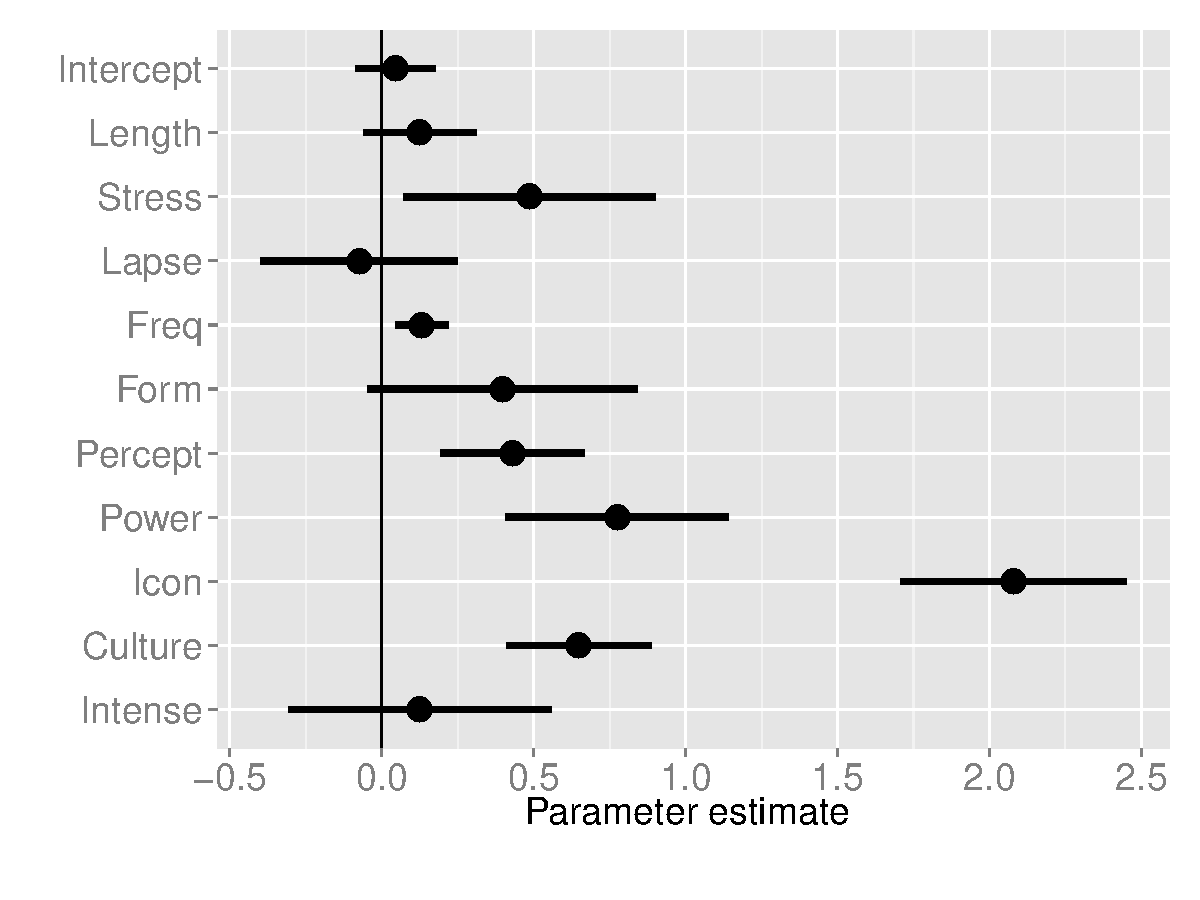
\includegraphics[scale=.35]{model-random.pdf}\vspace{-10pt}\label{fig:m-random}}\\
%\subfigure[][Beta-binomial model]{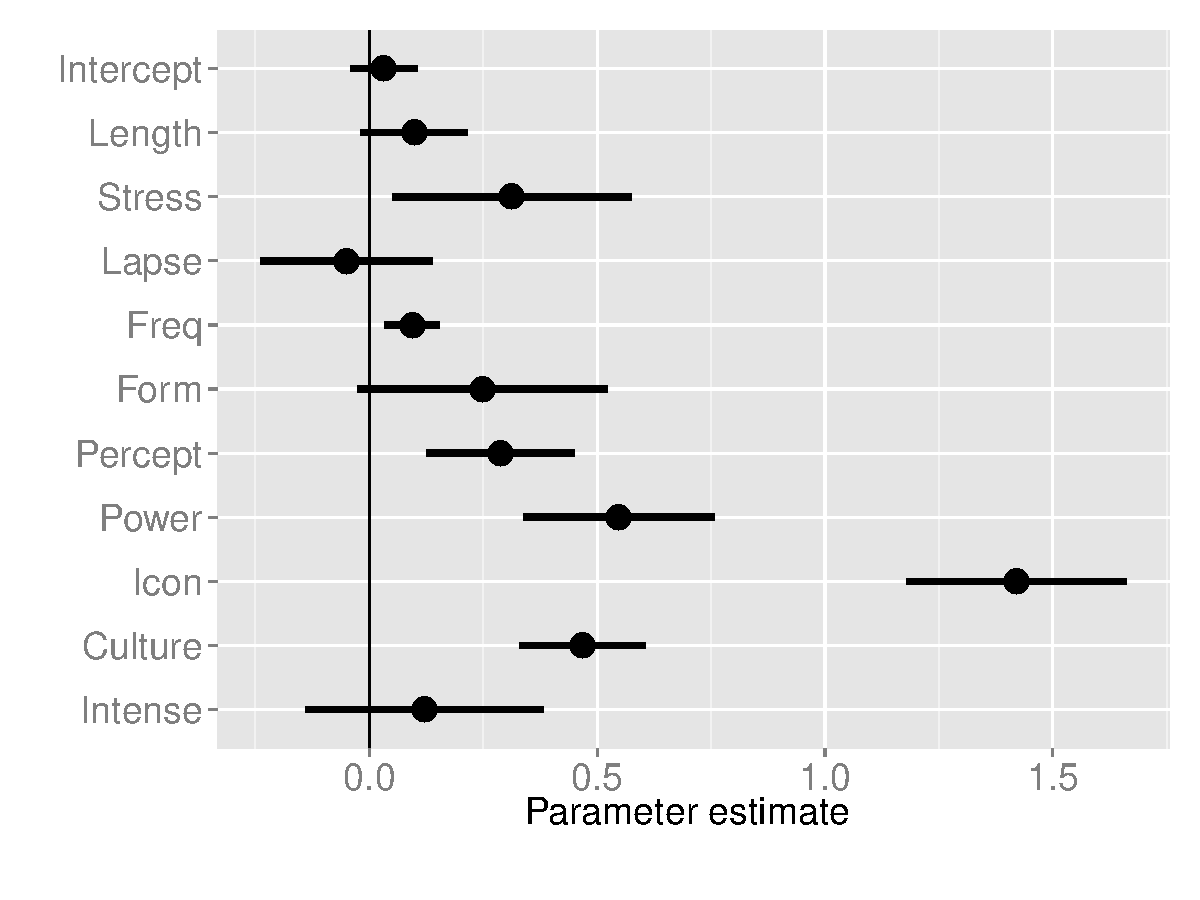
\includegraphics[scale=.35]{model-betabin.pdf}\label{fig:m-logistic}}
%\subfigure[][Beta-binomial model with variable concentration]{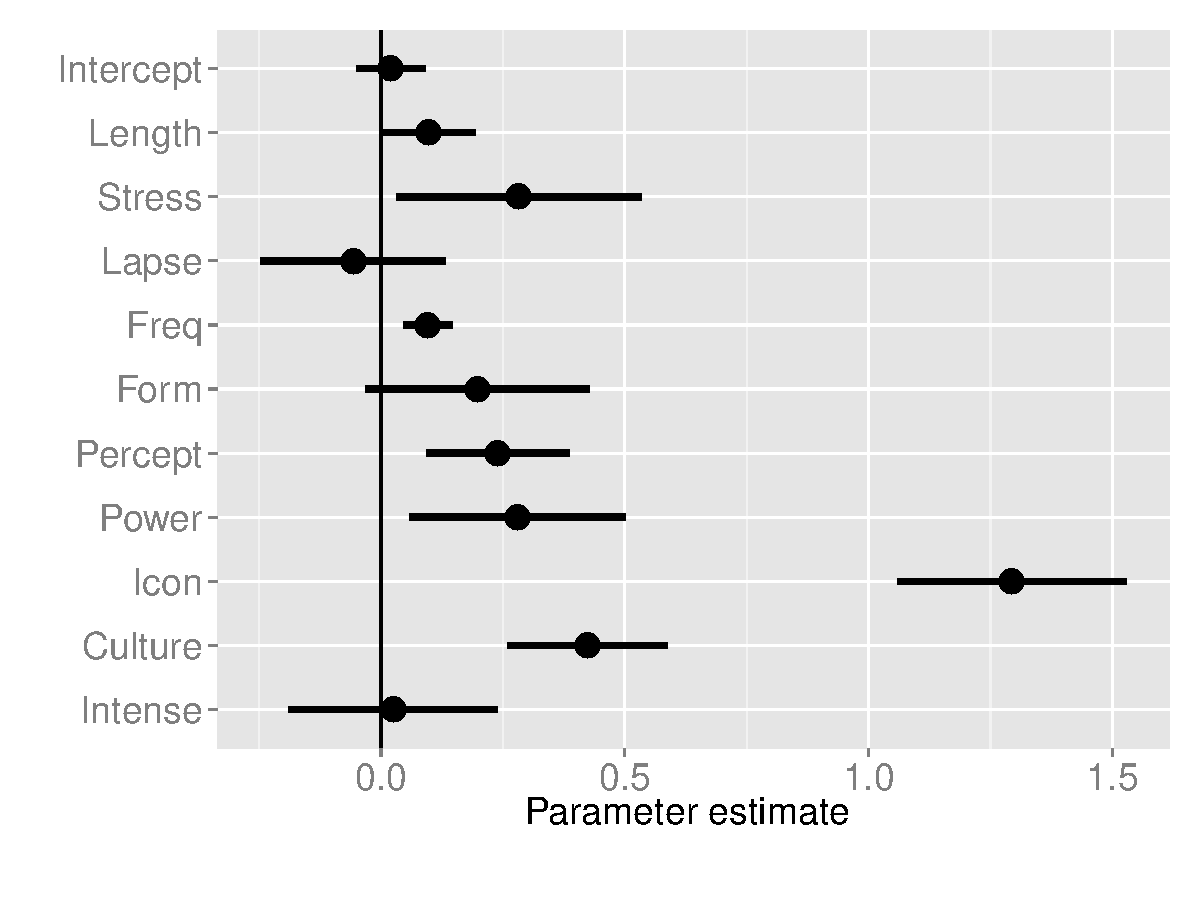
\includegraphics[scale=.35]{model-betabin-nu.pdf}\label{fig:m-random}}
%\vspace{-10pt}
%\caption{Parameter estimates for the logistic regression component of all four models. Dots show point estimates with bars indicating standard errors. TODO: Add error bars for all models}
%\label{fig:models}
%\end{figure*}

% TODO: redo these figures to include error bars for betabin models, and to change all the points to dots (regardless of significance). Make y.lab and y axis labels bigger

%\begin{table}[ht]
%\begin{center}
%\begin{tabular}{lrr}
% & L1 Err. (Std. Err.)& $R^{2}$\\\hline\hline
% Logistic & 0.169 (0.006) & 0.368\\
% Random intercept & 0.173 (0.006) & 0.355\\
% Beta-binomial & 0.172 (0.006) & 0.358\\
% Beta-binom w/ conc. & 0.168 (0.006) & 0.373
%\end{tabular}
%\end{center}
% \caption{Results from all models: mean by-type L1 error (with by-fold standard error), and $R^{2}$. The beta-binomial model with variable concentration parameter performs best on both metrics.}
% \label{t:L1}
%\end{table}

\subsection{Mixed-effects regression}
By far the most common method in language modeling for accounting for item-specific idiosyncrasies is mixed-effects regression models \citep{TFlorianJaeger:2008ev}. Formally, this model assumes that idiosyncratic preferences are distributed normally (in logit space) around the point estimate given by the fixed-effects components of the regression model.

We train a mixed-effect logistic regression on binomial tokens using the {\tt lme4} package in R. We use as predictors the same fixed effects as before, plus a random intercept for binomial types. As described above, the fitted model now predicts a \emph{distribution}, rather than a single point estimate, for a novel binomial. To make predictions for our (cross-validated) novel data, we sampled 1000 times from this distribution for each item. The histogram in Figure \ref{fig:models}(c) shows the full sample distribution across all items. In order to generate point estimate predictions for computing L1 and $R^{2}$ (shown in Figure \ref{fig:models}(b)), we take the sample median for each item, which optimizes the L1 error.

Including random intercepts improves neither our point estimates nor our language-wide distribution prediction. Apparently, the normal distribution of the random intercepts is not well suited to capturing the true distribution of binomial preferences. In particular, for a given item, the normality of random effects in \emph{logit} space leads to predictions that are skewed towards the extremities of \emph{probability} space.\footnote{An alternative method of prediction for novel items would be to take the median random intercept in logit space, i.e. to set all random intercepts to 0. This method yields results that are very similar to---but all-around slightly worse than---the original regression model.}


%\begin{figure}[h]
%\centering
%\subfigure{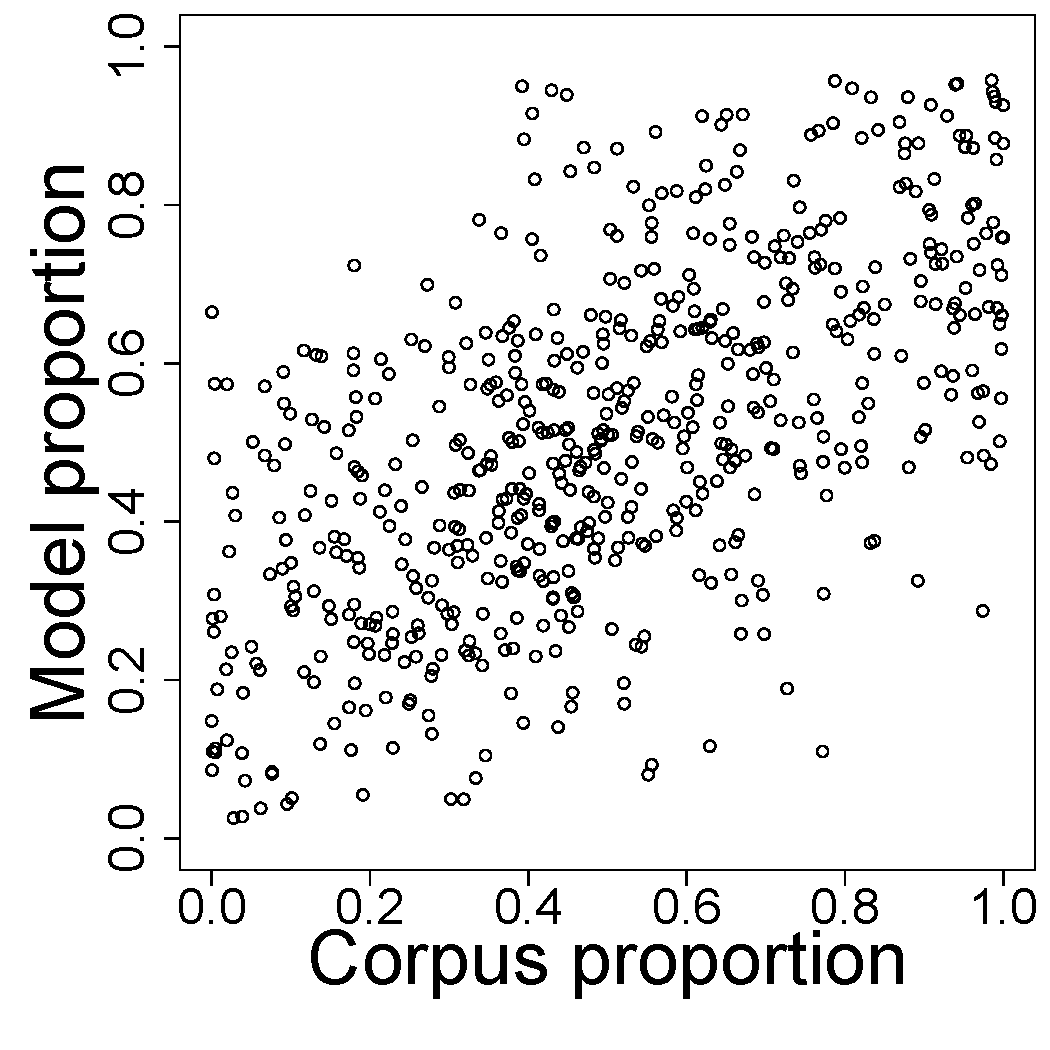
\includegraphics[scale=.25]{random-scatter.pdf}\label{fig:random-scatter}}
%\subfigure{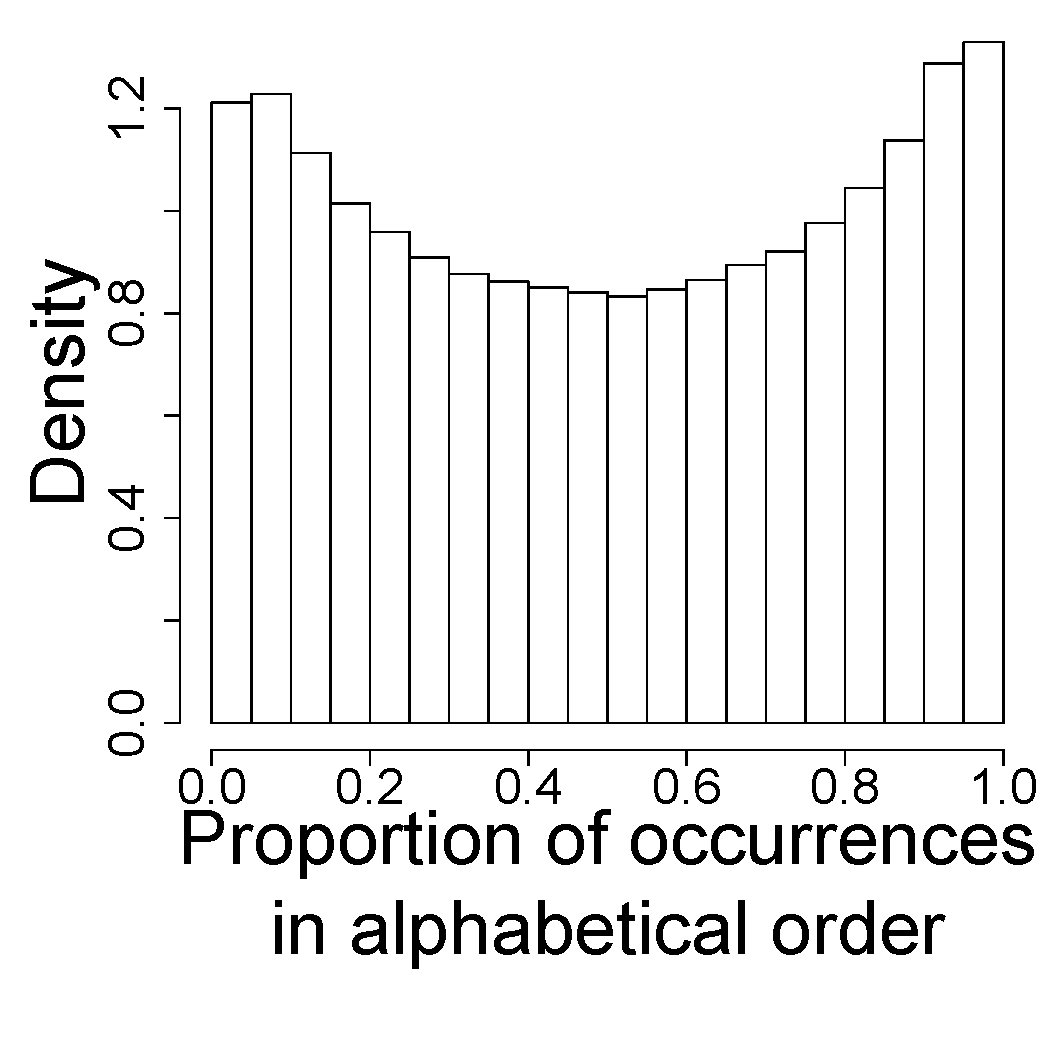
\includegraphics[scale=.2]{random-hist.pdf}\label{fig:random-hist}}
%\vspace{-10pt}
%\caption{Logistic regression with random intercept}
%\label{fig:random}
%\end{figure}
%

\subsection{Hierarchical Bayesian beta-binomial model}
Having seen that normally distributed random intercepts do not adequately capture the distribution of item-specific preferences, we introduce the beta distribution as a potentially better way to model this distribution. The beta distribution, defined on the interval $[0,1]$, has two parameters: one which determines the mean of the draws from the distribution, and one which determines the \emph{concentration}, i.e. whether draws are likely to be clustered around the mean versus distributed towards 0 and 1. For example, for a beta distribution with a mean of 0.7, a high concentration implies that most draws will be close to 0.7, while a low concentration implies that roughly 70\% of draws will be close to 1 and 30\% of draws will be close to 0. When we treat the output of the beta distribution as a predicted binomial preference, a high concentration corresponds to a pressure to maintain variation while a low concentration corresponds to a pressure to regularize.

In order to incorporate the beta distribution into our model of binomial preferences, we combine the logistic regression and the beta distribution in a hierarchical Bayesian model \citep{Gelman:2013un}, as shown in Figure \ref{fig:betabin}. For each item, the model determines a mean $\mu$ via standard logistic regression, using the same predictors as before. The model also fits a concentration parameter $\nu$. These two parameters determine a beta distribution from which the binomial preference $\pi$ is draw. Observed data is drawn from a binomial distribution with parameter $\pi$.

We fit this model using the {\tt rjags} package in {\tt R} \citep{Plummer:9TeVGfAZ}. After a burn-in period of 2000 iterations, we run for 2000 more iterations sampling every 20 iterations. In order to predict novel data, we fix the point estimates for the regression coefficients $\hat{\beta}$ and the concentration parameter $\nu$. We then sample 1000 draws of $\pi$ for each item. As with the mixed-effects model, the histogram in Figure \ref{fig:models}(c) shows the full sample distribution, while point estimates (the sample median) are used to calculate L1 error and $R^{2}$ (Figure \ref{fig:models}(b)).

This model performs better on L1 and $R^{2}$ than the mixed-effects model, but still worse than the initial logistic regression. The predicted histogram shows hints of the multimodal distribution seen in corpus data, but is overall too flat.

\begin{figure}
\centering
\subfigure{
\scalebox{0.6}{
\begin{pspicture}(1,-2)(6,6)
%\showgrid
\LARGE
% 2. Nodes
%%%%%%%%%%
% first row
\rput(2,6){\GM@node[nodeSize=11mm]{thetabeta}}
                 \GM@label[offset=-1.5mm]{thetabeta}{$\theta_\beta$}
               
\rput(2,4){\GM@node[nodeSize=11mm]{beta}}
                 \GM@label[offset=-1.5mm]{beta}{$\hat{\beta}$}
                 
\rput(4,4){\GM@node[nodeSize=11mm]{X}}
                 \GM@label[offset=-2mm]{X}{$\hat{X}$}
               
\rput(6,4){\GM@node[nodeSize=11mm]{thetanu}}
                 \GM@label[offset=-1.5mm]{thetanu}{$\theta_{\nu}$}
                 
%second row                                  
\rput(4,2){\GM@node[nodeSize=11mm]{mu}}
                 \GM@label[offset=-1.5mm]{mu}{$\mu$}
                                  
\rput(6,2){\GM@node[nodeSize=11mm]{nu}}
                 \GM@label[offset=-1.5mm]{nu}{$\nu$}



%third row                                  
\rput(4,0){\GM@node[nodeSize=11mm]{pi}}
                 \GM@label[offset=-1.5mm]{pi}{$\pi$}

%fourth row                                  
\rput(4,-2){\GM@node[nodeSize=11mm]{D}}
                 \GM@label[offset=-1.5mm]{D}{$D$}
                 
% 3. Arrows
%%%%%%%%%%%

\ncline[arrows=->]{thetabeta}{beta}
\ncline[arrows=->]{beta}{mu}
\ncline[arrows=->]{X}{mu}
\ncline[arrows=->]{thetanu}{nu}
\ncline[arrows=->]{mu}{pi}
\ncline[arrows=->]{nu}{pi}
\ncline[arrows=->]{pi}{D}

% 4. Plates
%%%%%%%%%%%

%\rput(1,3){\GM@plate[plateLabelPos=br]{4}{2}{P}}
\rput(3.25,-3.25){\GM@plate[plateLabelPos=br]{1.5}{2.25}{\normalsize$M_n$}}
\rput(3,-4){\GM@plate[plateLabelPos=br]{2}{9.5}{\normalsize$N$}}

\end{pspicture}
}}
\subfigure{
\begin{minipage}[b]{0.25\textwidth}
$N$: \# unordered binomial types\\
$M_n$: Frequency of binomial $n$\\
$\hat{X}$: Predictors (i.e. generative constraints)\\
$\hat{\beta}$: Regression coefficients\\
$\theta$: Uninformative priors\\
$\displaystyle \mu = \dfrac{1}{1 + e^{-\hat{X}\cdot\hat{\beta}}}$\\
$\nu \sim exp(\theta_\nu)$\\
$\pi\sim\text{Beta}(\mu,\nu)$\\
$D\sim\text{Binomial}(\pi,M_n)$
\end{minipage}
}
\caption{Our initial hierarchical Bayesian beta-binomial model. The set of nodes culiminating in $\mu$ implements a standard logistic regression. The output of this regression determines the mean of the beta distribution (with $\nu$ determining the concentration) from which $\pi$ and finally the observed data itself is drawn.}\label{fig:betabin}
\end{figure}

%\begin{figure}[h]
%\centering
%\subfigure{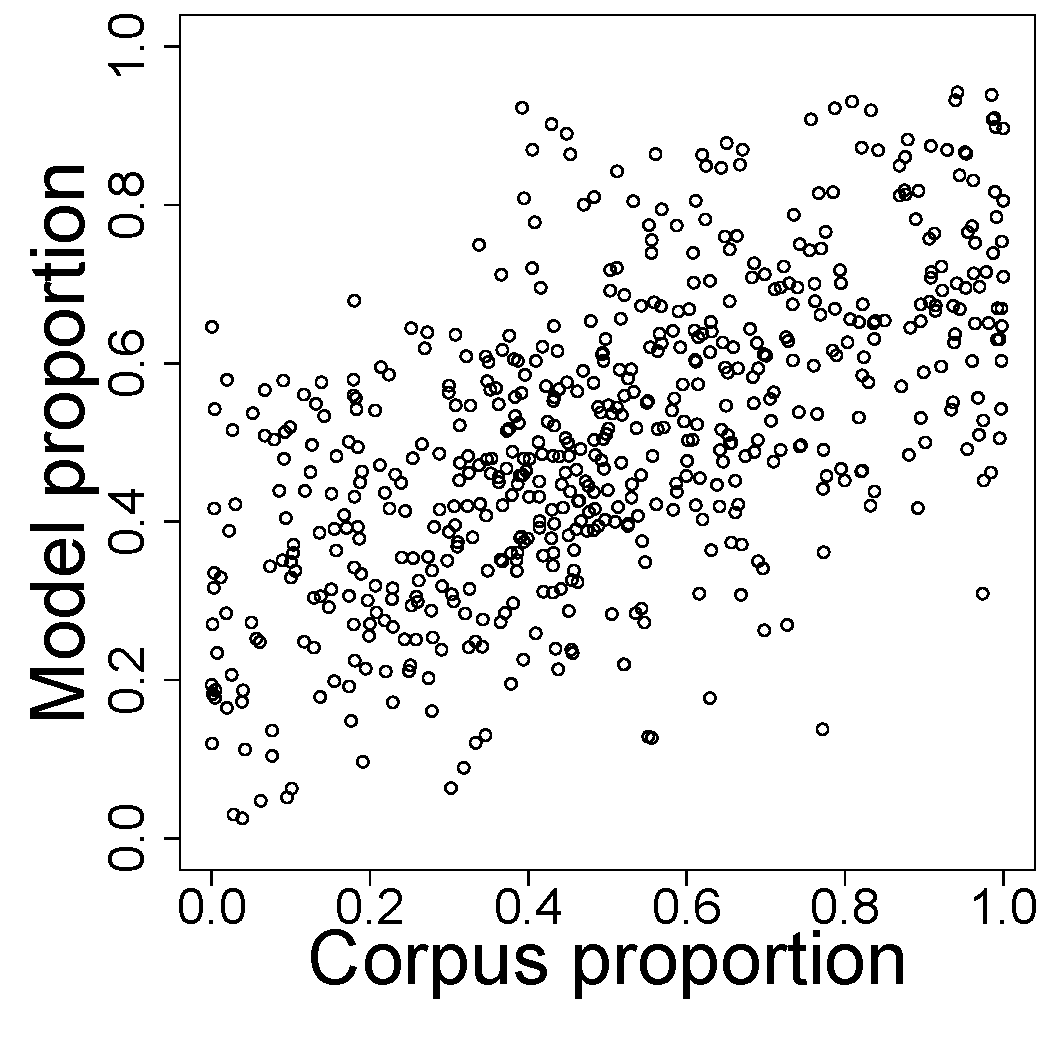
\includegraphics[scale=.25]{betabin-scatter.pdf}\label{fig:betabin-scatter}}
%\subfigure{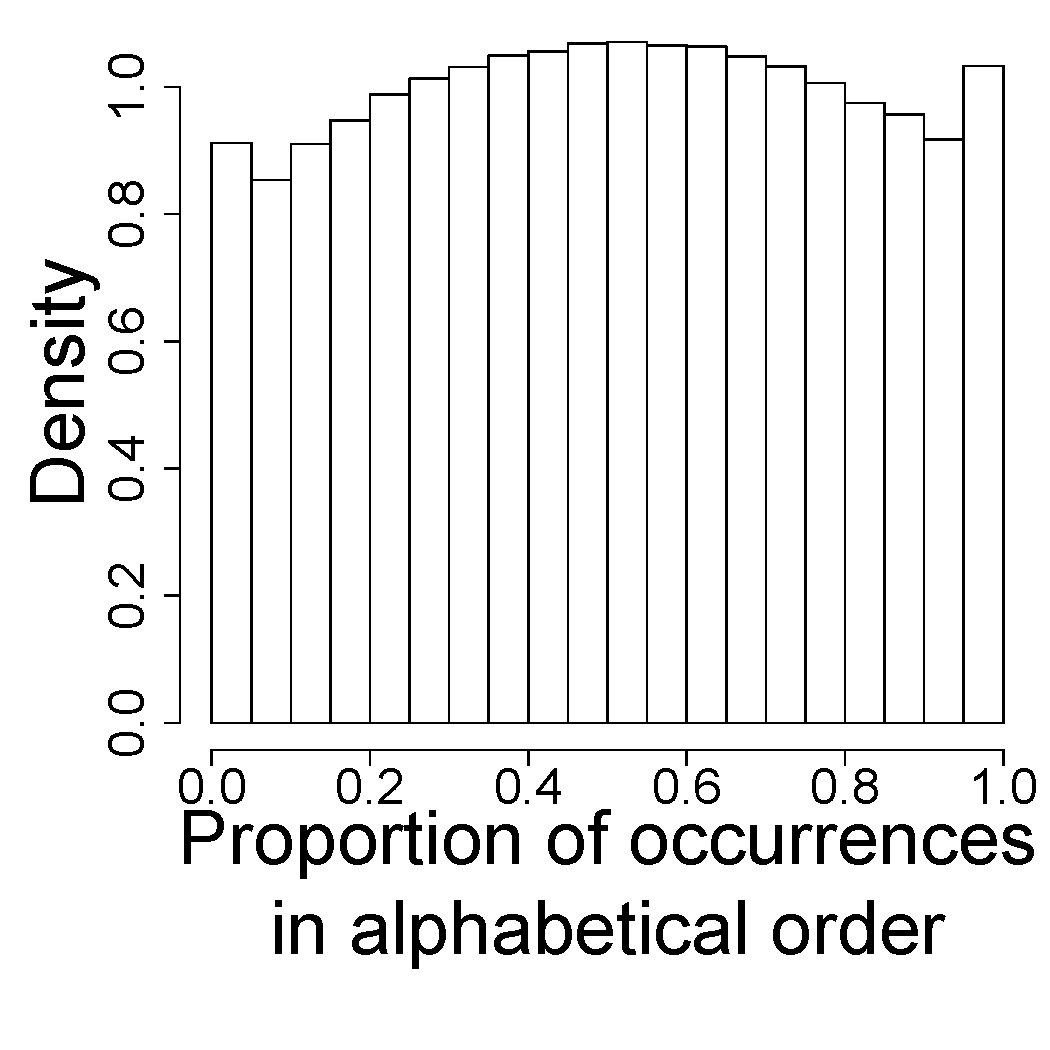
\includegraphics[scale=.2]{betabin-hist.pdf}\label{fig:betabin-hist}}
%\vspace{-10pt}
%\caption{Initial beta-binomial model results}
%\label{fig:betabin-results}
%\end{figure}



\subsection{Beta-binomial with a variable concentration parameter}
A crucial fact that we have not taken into account in previous models is the role of frequent reuse in shaping expressions' preferences. In particular, the degree to which an expression takes on a polarized preference may depend upon its frequency. We build upon the beta-binomial model in the previous section by parameterizing the concentration parameter by the frequency of the (unordered) binomial expression:
\begin{equation}\nu = exp(\alpha + \beta\cdot\text{log}(M_n))\end{equation}
where $M_n$ is the total number of occurrences of binomial $n$ in both orders. Training and testing of the model are identical to above.

We find that $\beta=-0.26$ is significantly different from 0 ($t_{99}=-94; p < 2.2\times 10^{-16}$), indicating that the concentration parameter changes significantly as a function of frequency: less frequent expressions have more dense distributions while more frequent expressions have more polarized distributions, as shown in Figure \ref{fig:nu}. We find that this model generates the best predictions of all our models, producing a marginally significant improvement in both L1 ($t_{593}=1.86; p = 0.06$) and $R^{2}$ (by fold $t_{19}=1.76; p = 0.09$) relative to the initial logistic regression. Moreover, it correctly predicts the multimodal distribution of expression preferences.

%\footnote{A version which fit the nu parameter with cubic splines rather than with this more constrained parameterization gave qualitatively and quantitatively similar results.}

\begin{figure}
\centering
\scalebox{0.6}{
\begin{pspicture}(1,-4)(10,6)
%\showgrid
\LARGE
% 2. Nodes
%%%%%%%%%%
% first row
\rput(2,6){\GM@node[nodeSize=11mm]{thetabeta}}
                 \GM@label[offset=-1.5mm]{thetabeta}{$\theta_\beta$}
               
\rput(2,4){\GM@node[nodeSize=11mm]{beta}}
                 \GM@label[offset=-1.5mm]{beta}{$\hat{\beta}$}
                 
\rput(4,4){\GM@node[nodeSize=11mm]{X}}
                 \GM@label[offset=-2mm]{X}{$\hat{X}$}
                 
\rput(6,4){\GM@node[nodeSize=11mm]{Mn}}
                 \GM@label[offset=-3mm]{Mn}{$M_n$}
                                  
\rput(8,6){\GM@node[nodeSize=11mm]{thetaab}}
                 \GM@label[offset=-3mm]{thetaab}{$\theta_{\alpha,\beta}$}
                 
%second row                                  
\rput(4,2){\GM@node[nodeSize=11mm]{mu}}
                 \GM@label[offset=-1.5mm]{mu}{$\mu$}
                                  
\rput(6,2){\GM@node[nodeSize=11mm]{nu}}
                 \GM@label[offset=-1.5mm]{nu}{$\nu$}

\rput(8,4){\GM@node[nodeSize=11mm]{ab}}
                 \GM@label[offset=-4mm]{ab}{$\alpha,\beta$}

%third row                                  
\rput(5,0){\GM@node[nodeSize=11mm]{pi}}
                 \GM@label[offset=-1.5mm]{pi}{$\pi$}

%fourth row                                  
\rput(5,-2){\GM@node[nodeSize=11mm]{D}}
                 \GM@label[offset=-1.5mm]{D}{$D$}
                 
% 3. Arrows
%%%%%%%%%%%

\ncline[arrows=->]{thetabeta}{beta}
\ncline[arrows=->]{beta}{mu}
\ncline[arrows=->]{X}{mu}
\ncline[arrows=->]{Mn}{nu}
\ncline[arrows=->]{thetaab}{ab}
\ncline[arrows=->]{ab}{nu}
\ncline[arrows=->]{mu}{pi}
\ncline[arrows=->]{nu}{pi}
\ncline[arrows=->]{pi}{D}

% 4. Plates
%%%%%%%%%%%

%\rput(1,3){\GM@plate[plateLabelPos=br]{4}{2}{P}}
\rput(4,-3){\GM@plate[plateLabelPos=br]{2}{2}{\normalsize$M_n$}}
\rput(3,-3.5){\GM@plate[plateLabelPos=br]{4}{8.5}{\normalsize$N$}}

\end{pspicture}
}
\caption{Hierarchical Bayesian beta-binomial model with variable concentration parameter}\label{fig:betabin-nu}
\end{figure}

%\begin{figure}[h]
%\centering
%\subfigure{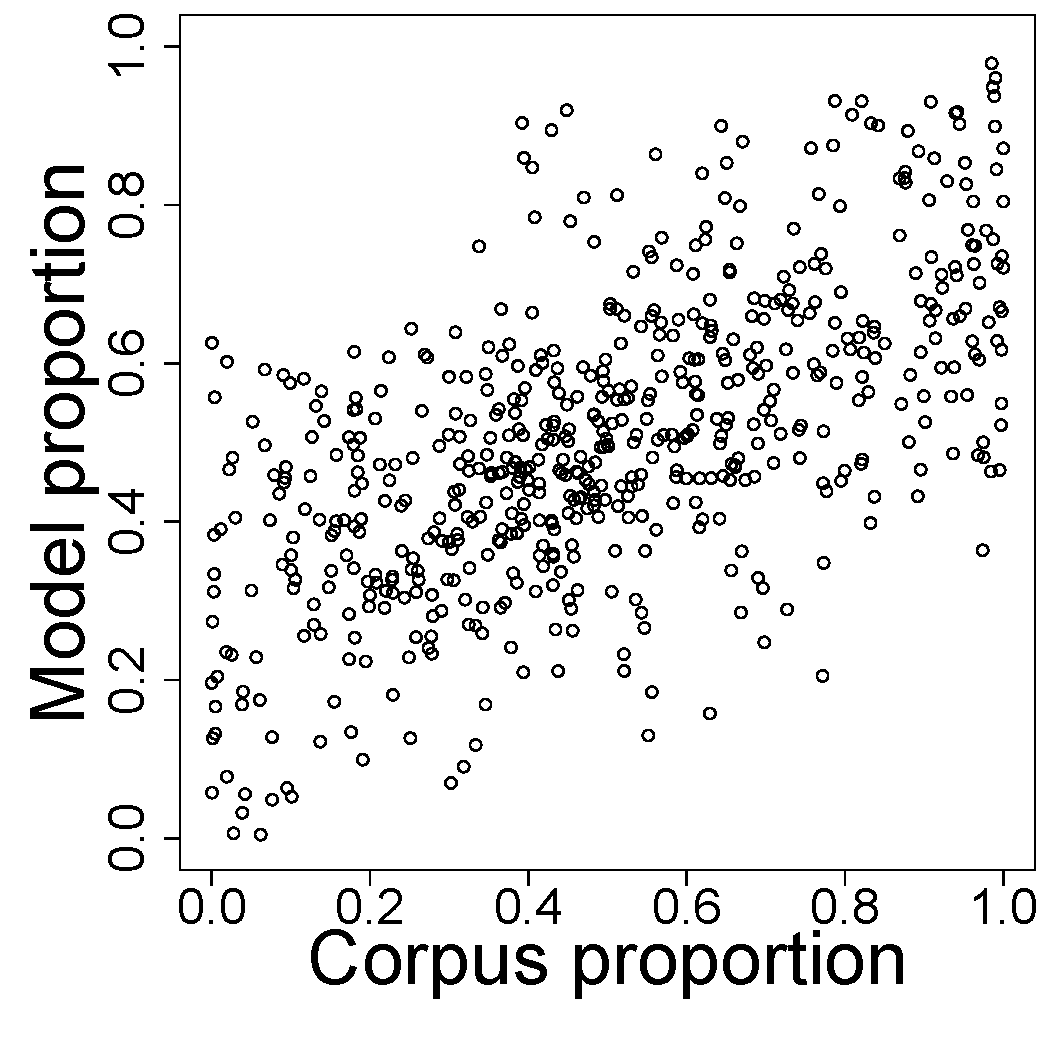
\includegraphics[scale=.25]{betabin-nu-scatter.pdf}\label{fig:betabin-nu-scatter}}
%\subfigure{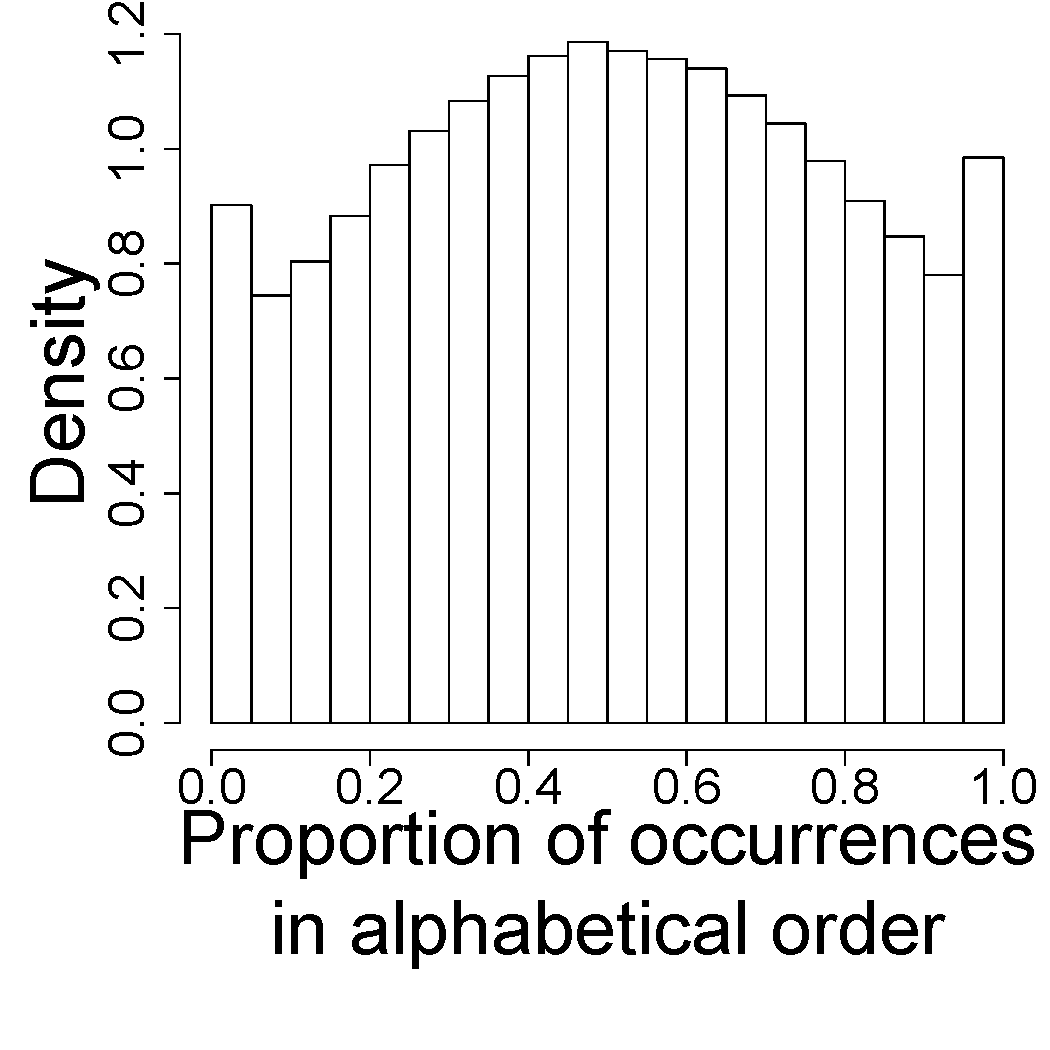
\includegraphics[scale=.2]{betabin-nu-hist.pdf}\label{fig:betabin-nu-hist}}
%\vspace{-10pt}
%\caption{Beta-binomial model with variable concentration parameter}
%\label{fig:betabin-nu-results}
%\end{figure}

\begin{figure}[h]
\centering
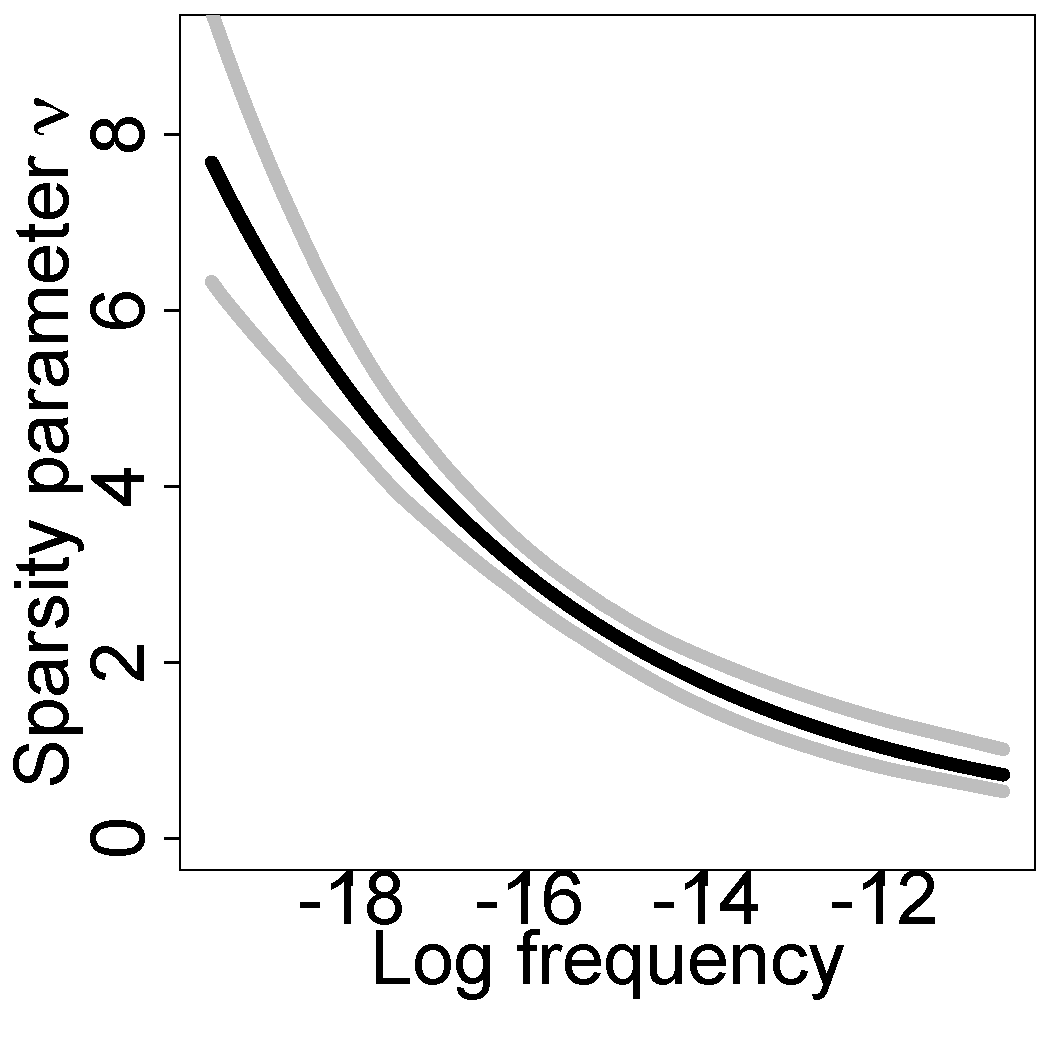
\includegraphics[scale=.2]{nu.pdf}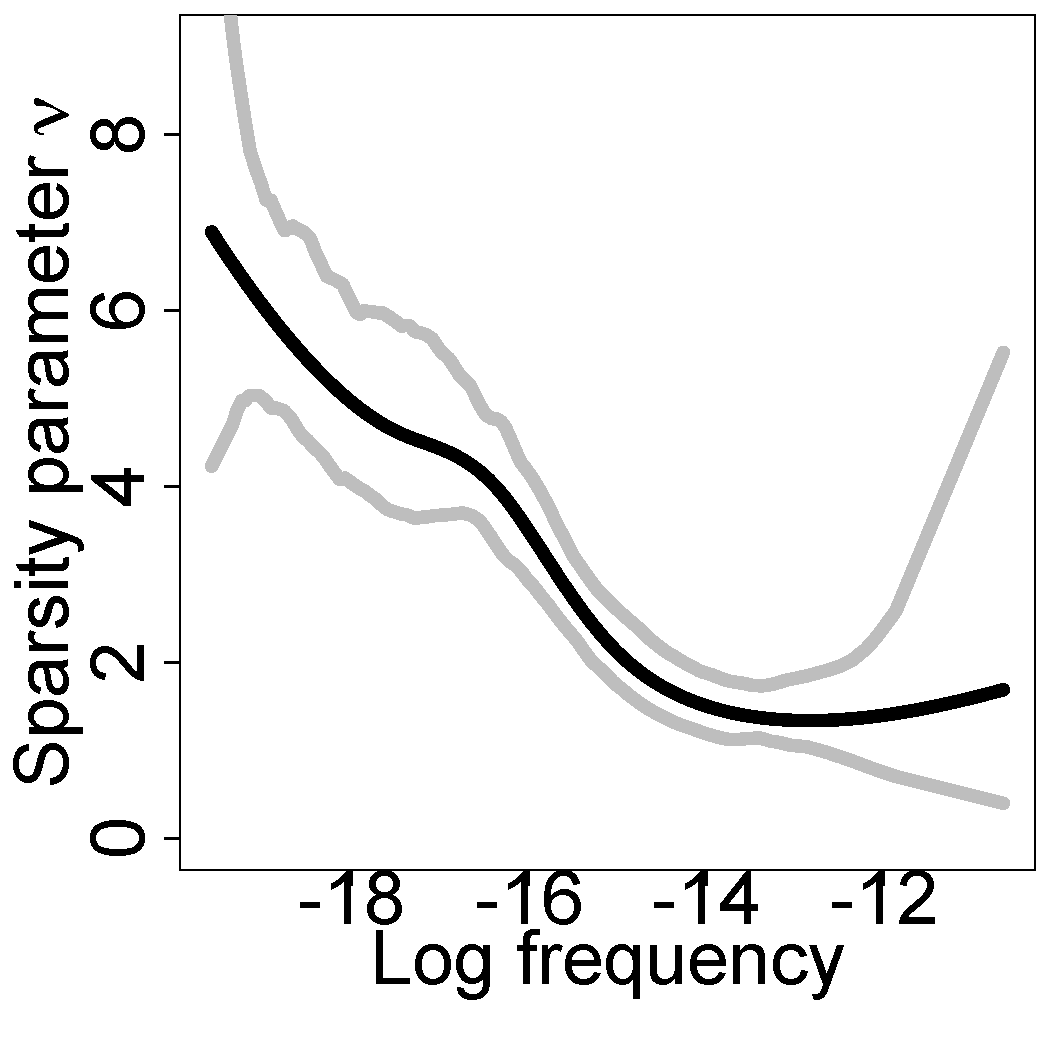
\includegraphics[scale=.2]{nu-splines.pdf}
\vspace{-10pt}
\caption{Concentration parameter $\nu$ as a function of frequency with 95\% confidence intervals. (Left) Parameterization given in Eq.\ 1. (Right) Alternate parameterization with cubic splines, for comparison.}
\label{fig:nu}
\end{figure}

\section{Discussion}
Overall, we found that all models made approximately similarly good best-guess predictions for binomials they weren't trained on, but the frequency-sensitive beta-binomial model was clearly superior in predicting the language-wide distribution of idiosyncratic binomial-specific ordering preferences. This model also indicates that more frequent binomials are on average more polarized.

This modeling finding supports \citet{Morgan:uMm0l0Ja}'s claim that generative knowledge and item-specific direct experience trade off gradiently in language processing, such that processing of novel or infrequent items relies upon generative knowledge, with reliance upon item-specific experience increasing with increasing frequency of exposure. \citeauthor{Morgan:uMm0l0Ja} support this claim with behavioral data, showing that empirical preferences for binomials which are completely novel depend on generative constraints while preferences for frequent expressions depend primarily on frequency of experience with each order. Our modeling results augment this argument by demonstrating that this trade-off is likewise necessary in order to predict the language-wide distribution of preference strengths. In particular, we can conceive of generative knowledge as providing a prior for ordering preferences. Under our final model, the logistic regression component serves an estimate of generative knowledge, which generates preferences clustered unimodally around 0.5. The amount of direct experience one has with an expression then modulates whether it conforms to this prior or whether it deviates. Items with low frequency have a high concentration: they maintain their variability and continue to contribute to the mode around 0.5. Items with high frequency have a low concentration: they are more likely to regularize and contribute to the modes at 0 and 1. Crucially, the inclusion of expression frequency as a predictor of the concentration of the beta distribution is necessary in order to achieve this effect in the model, demonstrating that expressions are indeed relying differentially on generative knowledge versus direct experience depending on their frequency.

This finding fits with previous models of cultural transmission in which, in general, preferences gravitate towards the prior \citep{Griffiths:2005wh}, but with sufficient exposure, exceptions can be learned \citep[e.g. irregular verbs;][]{Lieberman:2007bl}. However, this raises a question which is not answered by our or others' models: why don't all expressions converge to their prior preferences eventually? We present two possibilities.

One possibility is that people's probabilistic transmission behavior differs at different frequencies. Convergence to the prior relies upon \emph{probability matching}: people must reproduce variants in approximately the proportion in which they have encountered them. However, this is not the only possible behavior. Another possibility is that people preferentially reproduce the most frequent variant they have encountered, to the exclusion of all other variants, a process known as \emph{regularizing}. If people's tendency to probability match versus regularize is dependent on the frequency of the expression in question (with more regularizing at high frequencies), this could produce the pattern of more polarized expressions at higher frequencies seen in our data. Another possibility is that there is some other unspecified exogenous source of pressure towards regularization, as for instance seems to be the case in child language acquisition \citep{HudsonKam:2009vx}. This pressure might be weak enough that it is overwhelmed by convergence towards the prior at lower frequencies, but can be maintained for items with high enough frequencies to have sufficient exposure to deviate from the prior. Further work is necessary to disentangle these explanations.

In addition to contributing to our understanding of binomial expression processing, we have demonstrated the value of modeling the distribution of idiosyncratic preferences in two ways. First, it has improved our ability to predict preferences for novel items, by better differentiating the rule-following training data from the exceptions. Second, this model turns an observation about language-wide structure (the multimodal distribution of preferences) into a constraint on our theory of the cognitive representation and processing of language (more polarization at higher frequencies).

\section{Acknowledgments}
We gratefully acknowledge support from research grants NSF 0953870 and NICHD R01HD065829 and fellowships from the Alfred P. Sloan Foundation and the Center for Advanced Study in the Behavioral Sciences to Roger Levy.

\bibliographystyle{apacite}

\setlength{\bibleftmargin}{.125in}
\setlength{\bibindent}{3in}

\bibliography{bib}



\end{document}


%%%%%%%%%%%%%%%%%%%%%%%%%%%%%%%%%%%

\section{General Formatting Instructions}

The entire contribution of a proceedings paper (including figures,
references, and anything else) can be no longer than six pages.

The text of the paper should be formatted in two columns with an
overall width of 7 inches (17.8 cm) and length of 9.25 inches (23.5
cm), with 0.25 inches between the columns. Leave two line spaces
between the last author listed and the text of the paper. The left
margin should be 0.75 inches and the top margin should be 1 inch.
\textbf{The right and bottom margins will depend on whether you use
  U.S. letter or A4 paper, so you must be sure to measure the width of
  the printed text.} Use 10~point Times Roman with 12~point vertical
spacing, unless otherwise specified.

The title should be in 14~point, bold, and centered. The title should
be formatted with initial caps (the first letter of content words
capitalized and the rest lower case). Each author's name should appear
on a separate line, 11~point bold, and centered, with the author's
email address in parentheses. Under each author's name list the
author's affiliation and postal address in ordinary 10~point type.

Indent the first line of each paragraph by 1/8~inch (except for the
first paragraph of a new section). Do not add extra vertical space
between paragraphs.


\section{First Level Headings}

First level headings should be in 12~point, initial caps, bold and
centered. Leave one line space above the heading and 1/4~line space
below the heading.


\subsection{Second Level Headings}

Second level headings should be 11~point, initial caps, bold, and
flush left. Leave one line space above the heading and 1/4~line
space below the heading.


\subsubsection{Third Level Headings}

Third level headings should be 10~point, initial caps, bold, and flush
left. Leave one line space above the heading, but no space after the
heading.

\subsection{Footnotes}

Indicate footnotes with a number\footnote{Sample of the first
footnote.} in the text. Place the footnotes in 9~point type at the
bottom of the column on which they appear. Precede the footnote block
with a horizontal rule.\footnote{Sample of the second footnote.}


\subsection{Tables}

Number tables consecutively. Place the table number and title (in
10~point) above the table with one line space above the caption and
one line space below it, as in Table~\ref{sample-table}. You may float
tables to the top or bottom of a column, or set wide tables across
both columns.

\begin{table}[!ht]
\begin{center} 
\caption{Sample table title.} 
\label{sample-table} 
\vskip 0.12in
\begin{tabular}{ll} 
\hline
Error type    &  Example \\
\hline
Take smaller        &   63 - 44 = 21 \\
Always borrow~~~~   &   96 - 42 = 34 \\
0 - N = N           &   70 - 47 = 37 \\
0 - N = 0           &   70 - 47 = 30 \\
\hline
\end{tabular} 
\end{center} 
\end{table}


\subsection{Figures}

All artwork must be very dark for purposes of reproduction and should
not be hand drawn. Number figures sequentially, placing the figure
number and caption, in 10~point, after the figure with one line space
above the caption and one line space below it, as in
Figure~\ref{sample-figure}. If necessary, leave extra white space at
the bottom of the page to avoid splitting the figure and figure
caption. You may float figures to the top or bottom of a column, or
set wide figures across both columns.

\begin{figure}[ht]
\begin{center}
\fbox{CoGNiTiVe ScIeNcE}
\end{center}
\caption{This is a figure.} 
\label{sample-figure}
\end{figure}


\section{Acknowledgments}

Place acknowledgments (including funding information) in a section at
the end of the paper.


\section{References Instructions}

Follow the APA Publication Manual for citation format, both within the
text and in the reference list, with the following exceptions: (a) do
not cite the page numbers of any book, including chapters in edited
volumes; (b) use the same format for unpublished references as for
published ones. Alphabetize references by the surnames of the authors,
with single author entries preceding multiple author entries. Order
references by the same authors by the year of publication, with the
earliest first.

Use a first level section heading, ``{\bf References}'', as shown
below. Use a hanging indent style, with the first line of the
reference flush against the left margin and subsequent lines indented
by 1/8~inch. Below are example references for a conference paper, book
chapter, journal article, dissertation, book, technical report, and
edited volume, respectively.


